% Chapter 16: Review
% Statistics of Financial Markets -- Bachelor's programme, Bucharest University of Economic Studies
% GENERATED by latex/build_chapter16.py -- edit the generator, not this file.

\newcommand{\coursename}{Statistics of Financial Markets}
% Preambul comun SFM -- Statistica piețelor financiare / Statistics of Financial Markets (Beamer, 16:9)
% Același design ca MFM. Înainte de % Preambul comun SFM -- Statistica piețelor financiare / Statistics of Financial Markets (Beamer, 16:9)
% Același design ca MFM. Înainte de % Preambul comun SFM -- Statistica piețelor financiare / Statistics of Financial Markets (Beamer, 16:9)
% Același design ca MFM. Înainte de \input{../../latex/preamble} se definește
%   \newcommand{\coursename}{Statistics of Financial Markets}      (EN)
%   \newcommand{\coursename}{Statistica piețelor financiare}       (RO)  și  \def\sfmlang{ro}
% Fișierele .tex se află în EN/Courses, EN/Seminars, RO/Cursuri, RO/Seminarii (două niveluri sub rădăcină).
% Deck-urile sînt generate de latex/build_chapterN.py / build_seminarN.py (vezi latex/sfm_build.py).

\documentclass[9pt, aspectratio=169, t]{beamer}
\providecommand{\coursename}{Statistics of Financial Markets}

% Ensure content fits on slides
\setbeamersize{text margin left=8mm, text margin right=8mm}

%=============================================================================
% THEME AND STYLE CONFIGURATION
%=============================================================================
\usetheme{default}
% Using default theme for clean header/footer control

% Color Palette (matching Redispatch PDF)
\definecolor{MainBlue}{RGB}{26, 58, 110}
\definecolor{AccentBlue}{RGB}{26, 58, 110}
\definecolor{IDAred}{RGB}{205, 0, 0}
\definecolor{DarkGray}{RGB}{51, 51, 51}
\definecolor{MediumGray}{RGB}{128, 128, 128}
\definecolor{LightGray}{RGB}{248, 248, 248}
\definecolor{VeryLightGray}{RGB}{235, 235, 235}
\definecolor{KeynoteGray}{RGB}{218, 218, 218}
\definecolor{SectionGray}{RGB}{120, 120, 120}
\definecolor{FooterGray}{RGB}{100, 100, 100}
\definecolor{Crimson}{RGB}{220, 53, 69}
\definecolor{Forest}{RGB}{46, 125, 50}
\definecolor{Amber}{RGB}{181, 133, 63}
\definecolor{Orange}{RGB}{230, 126, 34}
\definecolor{Purple}{RGB}{142, 68, 173}

% Gradient background (exact Keynote 315° gradient: white to RGB 218,218,218)
\setbeamertemplate{background}{%
    \begin{tikzpicture}[remember picture, overlay]
        \shade[shading=axis, shading angle=315,
        top color=white, bottom color=KeynoteGray]
        (current page.south west) rectangle (current page.north east);
    \end{tikzpicture}%
}
% Fallback solid color for compatibility
\setbeamercolor{background canvas}{bg=}

\setbeamercolor{palette primary}{bg=MainBlue, fg=white}
\setbeamercolor{palette secondary}{bg=MainBlue!85, fg=white}
\setbeamercolor{palette tertiary}{bg=MainBlue!70, fg=white}
\setbeamercolor{structure}{fg=MainBlue}
\setbeamercolor{title}{fg=IDAred}
\setbeamercolor{frametitle}{fg=IDAred, bg=}
\setbeamercolor{block title}{bg=MainBlue, fg=white}
\setbeamercolor{block body}{bg=VeryLightGray, fg=DarkGray}
\setbeamercolor{block title alerted}{bg=Crimson, fg=white}
\setbeamercolor{block body alerted}{bg=Crimson!8, fg=DarkGray}
\setbeamercolor{block title example}{bg=Forest, fg=white}
\setbeamercolor{block body example}{bg=Forest!8, fg=DarkGray}
\setbeamercolor{item}{fg=MainBlue}

% Footer colors (override Madrid theme blue)
\setbeamercolor{author in head/foot}{fg=FooterGray, bg=}
\setbeamercolor{title in head/foot}{fg=FooterGray, bg=}
\setbeamercolor{date in head/foot}{fg=FooterGray, bg=}
\setbeamercolor{section in head/foot}{fg=FooterGray, bg=}
\setbeamercolor{subsection in head/foot}{fg=FooterGray, bg=}

% Bullet styles (apply everywhere including blocks)
\setbeamertemplate{itemize item}{\color{MainBlue}$\boxdot$}
\setbeamertemplate{itemize subitem}{\color{MainBlue}$\blacktriangleright$}
\setbeamertemplate{itemize subsubitem}{\color{MainBlue}\tiny$\bullet$}
\setbeamertemplate{itemize/enumerate body begin}{\normalsize}
\setbeamertemplate{itemize/enumerate subbody begin}{\normalsize}

% Item spacing - compact style
\setlength{\leftmargini}{10pt}       % Level 1: minimal indent
\setlength{\leftmarginii}{10pt}      % Level 2: minimal additional indent
% Compact list spacing (zero extra space before/after lists in blocks)
\makeatletter
\def\@listi{\leftmargin\leftmargini \topsep 0pt \parsep 0pt \itemsep 0pt}
\def\@listii{\leftmargin\leftmarginii \topsep 0pt \parsep 0pt \itemsep 0pt}
\makeatother

\setbeamertemplate{navigation symbols}{}

%=============================================================================
% CUSTOM HEADLINE
%=============================================================================
\setbeamertemplate{headline}{%
    \vskip10pt%
    \hbox to \paperwidth{%
        \hskip0.5cm%
        {\small\color{FooterGray}\renewcommand{\hyperlink}[2]{##2}\insertsectionhead}%
        \hfill%
        \textcolor{FooterGray}{\small\insertframenumber}%
        \hskip0.5cm%
    }%
    \vskip4pt%
    {\color{FooterGray}\hrule height 0.4pt}%
}

%=============================================================================
% CUSTOM FOOTER
%=============================================================================
\usepackage{fontawesome5}

\setbeamertemplate{footline}{%
    {\color{FooterGray}\hrule height 0.4pt}%
    \vskip4pt%
    \hbox to \paperwidth{%
        \hskip0.5cm%
        \textcolor{FooterGray}{\small\coursename}%
        \hfill%
        \raisebox{-0.1em}{%
            \begin{tikzpicture}[x=0.08em, y=0.08em, line width=0.4pt]
                \draw[FooterGray] (0,3) -- (1,4) -- (2,3.5) -- (3,5) -- (4,4) -- (5,6) -- (6,5.5) -- (7,4) -- (8,5) -- (9,7) -- (10,6) -- (11,5) -- (12,6.5) -- (13,8) -- (14,7) -- (15,6) -- (16,7.5) -- (17,9) -- (18,8) -- (19,7) -- (20,8.5) -- (21,10) -- (22,9) -- (23,8) -- (24,9.5);
            \end{tikzpicture}%
        }%
        \hskip0.5cm%
    }%
    \vskip6pt%
}

%=============================================================================
% PACKAGES
%=============================================================================
\usepackage[utf8]{inputenc}
\DeclareUnicodeCharacter{03B1}{\ensuremath{\alpha}}
\usepackage[T1]{fontenc}
\usepackage{amsmath, amssymb, amsthm}
\usepackage{mathtools}
\usepackage{bm}
\usepackage{tikz}
\usetikzlibrary{arrows.meta, positioning, shapes, calc, decorations.pathreplacing, shadings}
\usepackage{booktabs}
\usepackage{multirow}
\usepackage{array}
\usepackage{graphicx}
\usepackage{hyperref}
\usepackage{colortbl}
\usepackage{listings}
\lstset{language=Python, basicstyle=\ttfamily\scriptsize, keywordstyle=\color{MainBlue}\bfseries,
  commentstyle=\color{Forest}, stringstyle=\color{Crimson}, breaklines=true,
  frame=none, backgroundcolor=\color{VeryLightGray}, xleftmargin=2mm}
\hypersetup{colorlinks=true, linkcolor=MainBlue, urlcolor=MainBlue}
\graphicspath{{../../logos/}{../../charts/}{../../photos/}}
\usepackage{xcolor}
\hfuzz=2pt  % Suppress tiny overfull warnings (<2pt)
\vfuzz=2pt  % Suppress tiny vertical overfull warnings (<2pt)

%=============================================================================
% QUANTLET COMMANDS
%   \quantlet{<displayed name>}{<url>}       (generic, compatible with the older SFM decks)
%   \sfmquantlet{Ch_05}{SFM_ch5_garch}       -> https://github.com/danpele/SFM/tree/main/Quantlets/Ch_05/SFM_ch5_garch
%   \qlurl{<folder>} is defined per chapter by the generator (Quantlets/Ch_NN/<folder>)
%=============================================================================
\newcommand{\sfmrepo}{https://github.com/danpele/SFM}
\newcommand{\sfmqlbase}{https://github.com/danpele/SFM/tree/main/Quantlets}
\newcommand{\quantlet}[2]{%
    \hfill\href{#2}{%
        \raisebox{-0.15em}{
\includegraphics[height=0.7em]{ql_logo.png}}%
        \textcolor{MainBlue}{\tiny\ #1}%
    }%
}
\newcommand{\sfmquantlet}[2]{\quantlet{\detokenize{#2}}{\sfmqlbase/#1/#2}}

%=============================================================================
% NOTEBOOKS (Google Colab)
%   \colaburl{notebooks/EN/chapter5_seminar_notebook.ipynb} -> the Colab link of a file in the SFM repo
%   \nb: the chapter notebook (each seminar deck redefines it with \renewcommand)
%=============================================================================
\newcommand{\colaburl}[1]{https://colab.research.google.com/github/danpele/SFM/blob/main/#1}
\newcommand{\nb}{https://colab.research.google.com/github/danpele/SFM/tree/main/notebooks/EN}
\newcommand{\nbname}{notebooks/EN}

%=============================================================================
% SLIDE HELPERS (used by the generators; the same as in MFM)
%=============================================================================
% local font size for list bodies (the preamble forces \normalsize)
\newcommand{\itemsize}[1]{\setbeamertemplate{itemize/enumerate body begin}{#1}\setbeamertemplate{itemize/enumerate subbody begin}{#1}}
\newcommand{\intitle}[1]{{\hypersetup{urlcolor=white}#1}}   % white links inside coloured title bars
\newcommand{\imgcap}[1]{{\scriptsize #1}\\[0.5mm]}          % caption under a photo
\newcommand{\imgcredit}[2]{{\tiny\color{FooterGray}\href{#1}{#2}}}   % image credit: source URL, author/licence
\newcommand{\aiprompt}[1]{{\ttfamily\color{MainBlue}#1}}     % a prompt to an AI assistant

%=============================================================================
% SEMINARS: student version by default; the instructor wrapper *_solutions.tex sets \solutionstrue
%=============================================================================
\makeatletter\@ifundefined{ifsolutions}{\expandafter\newif\csname ifsolutions\endcsname}{}\makeatother
\newcommand{\solonly}[1]{\ifsolutions #1\fi}
\newcommand{\propsub}{\ifsolutions\else\framesubtitle{\ifdefined\sfmlang Rezolvarea se discută la seminar\else Solution discussed in class\fi}\fi}

%=============================================================================
% APPENDIX AND CHAPTER LINKS (latex/appendix_links.py writes the calls; it also re-declares these
% macros before \begin{document}, so the decks compile with or without this preamble block)
%=============================================================================
\providecommand{\sfmapplink}[3]{\hypertarget{#2}{}\hyperlink{#1}{\beamergotobutton{#3}}}
\providecommand{\sfmappback}[2]{\begin{tikzpicture}[remember picture,overlay]\node[anchor=south east] at ([xshift=-3mm,yshift=7mm]current page.south east){\hyperlink{#1}{\beamerreturnbutton{#2}}};\end{tikzpicture}}
\providecommand{\sfmchlink}[2]{\href{#1}{#2}}
\providecommand{\sfmchlinkt}[2]{\href{#1}{\usebeamercolor[fg]{frametitle}#2}}

%=============================================================================
% QUANTINAR COMMAND: link către un curs Quantinar (subiecte avansate)
%=============================================================================
\newcommand{\quantinar}[2]{%
    \href{#2}{%
        \raisebox{-0.15em}{
\includegraphics[height=0.8em]{qr_logo.png}}%
        \textcolor{MainBlue}{\scriptsize\ #1}%
    }%
}

%=============================================================================
% CUSTOM TITLE PAGE
%=============================================================================
\defbeamertemplate*{title page}{hybrid}[1][]
{
    \vspace{0.2cm}
    % Logos row - top header (with clickable links)
    \begin{center}
        \href{https://www.ase.ro}{
\includegraphics[height=1.0cm]{ase_logo.png}}\hspace{0.3cm}%
        \href{https://theida.net}{
\includegraphics[height=1.0cm]{ida_logo.png}}\hspace{0.3cm}%
        \href{https://blockchain-research-center.com}{
\includegraphics[height=1.0cm]{brc_logo.png}}\hspace{0.3cm}%
        \href{https://www.ai4efin.ase.ro}{
\includegraphics[height=1.0cm]{ai4efin_logo.png}}\hspace{0.3cm}%
        \href{https://ipe.ro/new}{
\includegraphics[height=1.0cm]{acad_logo.png}}\hspace{0.3cm}%
        \href{https://www.digital-finance-msca.com}{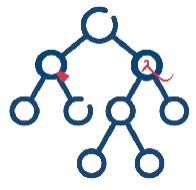
\includegraphics[height=1.0cm]{msca_logo.png}}%
    \end{center}

    \vspace{0.6cm}

    % Main title with Q logos on sides (with clickable links)
    \begin{center}
        \begin{minipage}{0.1\textwidth}
            \centering
            \href{https://quantlet.com}{
\includegraphics[height=1.1cm]{ql_logo.png}}
        \end{minipage}%
        \begin{minipage}{0.78\textwidth}
            \centering
            {\LARGE\bfseries\usebeamercolor[fg]{title}\inserttitle}

            \vspace{0.3cm}

            {\usebeamerfont{subtitle}\usebeamercolor[fg]{title}\insertsubtitle}
        \end{minipage}%
        \begin{minipage}{0.1\textwidth}
            \centering
            \href{https://quantinar.com}{
\includegraphics[height=1.1cm]{qr_logo.png}}
        \end{minipage}
    \end{center}

    \vspace{0.6cm}

    % Authors (left aligned)
    \hspace{0.5cm}{\usebeamerfont{author}\insertauthor}

    \vspace{0.3cm}

    % Institute/Affiliations (left aligned)
    \hspace{0.5cm}\begin{minipage}[t]{0.9\textwidth}
        \raggedright\small\insertinstitute
    \end{minipage}
}

%=============================================================================
% THEOREM ENVIRONMENTS
%=============================================================================
\theoremstyle{definition}
\setbeamertemplate{theorems}[numbered]
\ifdefined\sfmlang
\newtheorem{defn}{Definiție}
\newtheorem{thm}{Teoremă}
\newtheorem{prop}{Propoziție}
\newtheorem{rmk}{Observație}
\else
\newtheorem{defn}{Definition}
\newtheorem{thm}{Theorem}
\newtheorem{prop}{Proposition}
\newtheorem{rmk}{Remark}
\fi

%=============================================================================
% CENTRED MINIPAGE (no extra vertical space)
%=============================================================================
\newenvironment{cminipage}[1]{%
    \par\noindent\hfill\begin{minipage}{#1}\ignorespaces
}{%
    \end{minipage}\hfill\null\par
}

%=============================================================================
% CUSTOM COMMANDS
%=============================================================================
\newcommand{\E}{\mathbb{E}}
\newcommand{\Var}{\text{Var}}
\newcommand{\Cov}{\text{Cov}}
\newcommand{\Corr}{\text{Corr}}
\newcommand{\R}{\mathbb{R}}
\newcommand{\N}{\mathbb{N}}
\newcommand{\Z}{\mathbb{Z}}
\newcommand{\B}{\mathbf{B}}
\newcommand{\imark}{\textcolor{MainBlue}{\textbullet}}
\newcommand{\RMSE}{\text{RMSE}}
\newcommand{\MAE}{\text{MAE}}
\newcommand{\MAPE}{\text{MAPE}}

 se definește
%   \newcommand{\coursename}{Statistics of Financial Markets}      (EN)
%   \newcommand{\coursename}{Statistica piețelor financiare}       (RO)  și  \def\sfmlang{ro}
% Fișierele .tex se află în EN/Courses, EN/Seminars, RO/Cursuri, RO/Seminarii (două niveluri sub rădăcină).
% Deck-urile sînt generate de latex/build_chapterN.py / build_seminarN.py (vezi latex/sfm_build.py).

\documentclass[9pt, aspectratio=169, t]{beamer}
\providecommand{\coursename}{Statistics of Financial Markets}

% Ensure content fits on slides
\setbeamersize{text margin left=8mm, text margin right=8mm}

%=============================================================================
% THEME AND STYLE CONFIGURATION
%=============================================================================
\usetheme{default}
% Using default theme for clean header/footer control

% Color Palette (matching Redispatch PDF)
\definecolor{MainBlue}{RGB}{26, 58, 110}
\definecolor{AccentBlue}{RGB}{26, 58, 110}
\definecolor{IDAred}{RGB}{205, 0, 0}
\definecolor{DarkGray}{RGB}{51, 51, 51}
\definecolor{MediumGray}{RGB}{128, 128, 128}
\definecolor{LightGray}{RGB}{248, 248, 248}
\definecolor{VeryLightGray}{RGB}{235, 235, 235}
\definecolor{KeynoteGray}{RGB}{218, 218, 218}
\definecolor{SectionGray}{RGB}{120, 120, 120}
\definecolor{FooterGray}{RGB}{100, 100, 100}
\definecolor{Crimson}{RGB}{220, 53, 69}
\definecolor{Forest}{RGB}{46, 125, 50}
\definecolor{Amber}{RGB}{181, 133, 63}
\definecolor{Orange}{RGB}{230, 126, 34}
\definecolor{Purple}{RGB}{142, 68, 173}

% Gradient background (exact Keynote 315° gradient: white to RGB 218,218,218)
\setbeamertemplate{background}{%
    \begin{tikzpicture}[remember picture, overlay]
        \shade[shading=axis, shading angle=315,
        top color=white, bottom color=KeynoteGray]
        (current page.south west) rectangle (current page.north east);
    \end{tikzpicture}%
}
% Fallback solid color for compatibility
\setbeamercolor{background canvas}{bg=}

\setbeamercolor{palette primary}{bg=MainBlue, fg=white}
\setbeamercolor{palette secondary}{bg=MainBlue!85, fg=white}
\setbeamercolor{palette tertiary}{bg=MainBlue!70, fg=white}
\setbeamercolor{structure}{fg=MainBlue}
\setbeamercolor{title}{fg=IDAred}
\setbeamercolor{frametitle}{fg=IDAred, bg=}
\setbeamercolor{block title}{bg=MainBlue, fg=white}
\setbeamercolor{block body}{bg=VeryLightGray, fg=DarkGray}
\setbeamercolor{block title alerted}{bg=Crimson, fg=white}
\setbeamercolor{block body alerted}{bg=Crimson!8, fg=DarkGray}
\setbeamercolor{block title example}{bg=Forest, fg=white}
\setbeamercolor{block body example}{bg=Forest!8, fg=DarkGray}
\setbeamercolor{item}{fg=MainBlue}

% Footer colors (override Madrid theme blue)
\setbeamercolor{author in head/foot}{fg=FooterGray, bg=}
\setbeamercolor{title in head/foot}{fg=FooterGray, bg=}
\setbeamercolor{date in head/foot}{fg=FooterGray, bg=}
\setbeamercolor{section in head/foot}{fg=FooterGray, bg=}
\setbeamercolor{subsection in head/foot}{fg=FooterGray, bg=}

% Bullet styles (apply everywhere including blocks)
\setbeamertemplate{itemize item}{\color{MainBlue}$\boxdot$}
\setbeamertemplate{itemize subitem}{\color{MainBlue}$\blacktriangleright$}
\setbeamertemplate{itemize subsubitem}{\color{MainBlue}\tiny$\bullet$}
\setbeamertemplate{itemize/enumerate body begin}{\normalsize}
\setbeamertemplate{itemize/enumerate subbody begin}{\normalsize}

% Item spacing - compact style
\setlength{\leftmargini}{10pt}       % Level 1: minimal indent
\setlength{\leftmarginii}{10pt}      % Level 2: minimal additional indent
% Compact list spacing (zero extra space before/after lists in blocks)
\makeatletter
\def\@listi{\leftmargin\leftmargini \topsep 0pt \parsep 0pt \itemsep 0pt}
\def\@listii{\leftmargin\leftmarginii \topsep 0pt \parsep 0pt \itemsep 0pt}
\makeatother

\setbeamertemplate{navigation symbols}{}

%=============================================================================
% CUSTOM HEADLINE
%=============================================================================
\setbeamertemplate{headline}{%
    \vskip10pt%
    \hbox to \paperwidth{%
        \hskip0.5cm%
        {\small\color{FooterGray}\renewcommand{\hyperlink}[2]{##2}\insertsectionhead}%
        \hfill%
        \textcolor{FooterGray}{\small\insertframenumber}%
        \hskip0.5cm%
    }%
    \vskip4pt%
    {\color{FooterGray}\hrule height 0.4pt}%
}

%=============================================================================
% CUSTOM FOOTER
%=============================================================================
\usepackage{fontawesome5}

\setbeamertemplate{footline}{%
    {\color{FooterGray}\hrule height 0.4pt}%
    \vskip4pt%
    \hbox to \paperwidth{%
        \hskip0.5cm%
        \textcolor{FooterGray}{\small\coursename}%
        \hfill%
        \raisebox{-0.1em}{%
            \begin{tikzpicture}[x=0.08em, y=0.08em, line width=0.4pt]
                \draw[FooterGray] (0,3) -- (1,4) -- (2,3.5) -- (3,5) -- (4,4) -- (5,6) -- (6,5.5) -- (7,4) -- (8,5) -- (9,7) -- (10,6) -- (11,5) -- (12,6.5) -- (13,8) -- (14,7) -- (15,6) -- (16,7.5) -- (17,9) -- (18,8) -- (19,7) -- (20,8.5) -- (21,10) -- (22,9) -- (23,8) -- (24,9.5);
            \end{tikzpicture}%
        }%
        \hskip0.5cm%
    }%
    \vskip6pt%
}

%=============================================================================
% PACKAGES
%=============================================================================
\usepackage[utf8]{inputenc}
\DeclareUnicodeCharacter{03B1}{\ensuremath{\alpha}}
\usepackage[T1]{fontenc}
\usepackage{amsmath, amssymb, amsthm}
\usepackage{mathtools}
\usepackage{bm}
\usepackage{tikz}
\usetikzlibrary{arrows.meta, positioning, shapes, calc, decorations.pathreplacing, shadings}
\usepackage{booktabs}
\usepackage{multirow}
\usepackage{array}
\usepackage{graphicx}
\usepackage{hyperref}
\usepackage{colortbl}
\usepackage{listings}
\lstset{language=Python, basicstyle=\ttfamily\scriptsize, keywordstyle=\color{MainBlue}\bfseries,
  commentstyle=\color{Forest}, stringstyle=\color{Crimson}, breaklines=true,
  frame=none, backgroundcolor=\color{VeryLightGray}, xleftmargin=2mm}
\hypersetup{colorlinks=true, linkcolor=MainBlue, urlcolor=MainBlue}
\graphicspath{{../../logos/}{../../charts/}{../../photos/}}
\usepackage{xcolor}
\hfuzz=2pt  % Suppress tiny overfull warnings (<2pt)
\vfuzz=2pt  % Suppress tiny vertical overfull warnings (<2pt)

%=============================================================================
% QUANTLET COMMANDS
%   \quantlet{<displayed name>}{<url>}       (generic, compatible with the older SFM decks)
%   \sfmquantlet{Ch_05}{SFM_ch5_garch}       -> https://github.com/danpele/SFM/tree/main/Quantlets/Ch_05/SFM_ch5_garch
%   \qlurl{<folder>} is defined per chapter by the generator (Quantlets/Ch_NN/<folder>)
%=============================================================================
\newcommand{\sfmrepo}{https://github.com/danpele/SFM}
\newcommand{\sfmqlbase}{https://github.com/danpele/SFM/tree/main/Quantlets}
\newcommand{\quantlet}[2]{%
    \hfill\href{#2}{%
        \raisebox{-0.15em}{
\includegraphics[height=0.7em]{ql_logo.png}}%
        \textcolor{MainBlue}{\tiny\ #1}%
    }%
}
\newcommand{\sfmquantlet}[2]{\quantlet{\detokenize{#2}}{\sfmqlbase/#1/#2}}

%=============================================================================
% NOTEBOOKS (Google Colab)
%   \colaburl{notebooks/EN/chapter5_seminar_notebook.ipynb} -> the Colab link of a file in the SFM repo
%   \nb: the chapter notebook (each seminar deck redefines it with \renewcommand)
%=============================================================================
\newcommand{\colaburl}[1]{https://colab.research.google.com/github/danpele/SFM/blob/main/#1}
\newcommand{\nb}{https://colab.research.google.com/github/danpele/SFM/tree/main/notebooks/EN}
\newcommand{\nbname}{notebooks/EN}

%=============================================================================
% SLIDE HELPERS (used by the generators; the same as in MFM)
%=============================================================================
% local font size for list bodies (the preamble forces \normalsize)
\newcommand{\itemsize}[1]{\setbeamertemplate{itemize/enumerate body begin}{#1}\setbeamertemplate{itemize/enumerate subbody begin}{#1}}
\newcommand{\intitle}[1]{{\hypersetup{urlcolor=white}#1}}   % white links inside coloured title bars
\newcommand{\imgcap}[1]{{\scriptsize #1}\\[0.5mm]}          % caption under a photo
\newcommand{\imgcredit}[2]{{\tiny\color{FooterGray}\href{#1}{#2}}}   % image credit: source URL, author/licence
\newcommand{\aiprompt}[1]{{\ttfamily\color{MainBlue}#1}}     % a prompt to an AI assistant

%=============================================================================
% SEMINARS: student version by default; the instructor wrapper *_solutions.tex sets \solutionstrue
%=============================================================================
\makeatletter\@ifundefined{ifsolutions}{\expandafter\newif\csname ifsolutions\endcsname}{}\makeatother
\newcommand{\solonly}[1]{\ifsolutions #1\fi}
\newcommand{\propsub}{\ifsolutions\else\framesubtitle{\ifdefined\sfmlang Rezolvarea se discută la seminar\else Solution discussed in class\fi}\fi}

%=============================================================================
% APPENDIX AND CHAPTER LINKS (latex/appendix_links.py writes the calls; it also re-declares these
% macros before \begin{document}, so the decks compile with or without this preamble block)
%=============================================================================
\providecommand{\sfmapplink}[3]{\hypertarget{#2}{}\hyperlink{#1}{\beamergotobutton{#3}}}
\providecommand{\sfmappback}[2]{\begin{tikzpicture}[remember picture,overlay]\node[anchor=south east] at ([xshift=-3mm,yshift=7mm]current page.south east){\hyperlink{#1}{\beamerreturnbutton{#2}}};\end{tikzpicture}}
\providecommand{\sfmchlink}[2]{\href{#1}{#2}}
\providecommand{\sfmchlinkt}[2]{\href{#1}{\usebeamercolor[fg]{frametitle}#2}}

%=============================================================================
% QUANTINAR COMMAND: link către un curs Quantinar (subiecte avansate)
%=============================================================================
\newcommand{\quantinar}[2]{%
    \href{#2}{%
        \raisebox{-0.15em}{
\includegraphics[height=0.8em]{qr_logo.png}}%
        \textcolor{MainBlue}{\scriptsize\ #1}%
    }%
}

%=============================================================================
% CUSTOM TITLE PAGE
%=============================================================================
\defbeamertemplate*{title page}{hybrid}[1][]
{
    \vspace{0.2cm}
    % Logos row - top header (with clickable links)
    \begin{center}
        \href{https://www.ase.ro}{
\includegraphics[height=1.0cm]{ase_logo.png}}\hspace{0.3cm}%
        \href{https://theida.net}{
\includegraphics[height=1.0cm]{ida_logo.png}}\hspace{0.3cm}%
        \href{https://blockchain-research-center.com}{
\includegraphics[height=1.0cm]{brc_logo.png}}\hspace{0.3cm}%
        \href{https://www.ai4efin.ase.ro}{
\includegraphics[height=1.0cm]{ai4efin_logo.png}}\hspace{0.3cm}%
        \href{https://ipe.ro/new}{
\includegraphics[height=1.0cm]{acad_logo.png}}\hspace{0.3cm}%
        \href{https://www.digital-finance-msca.com}{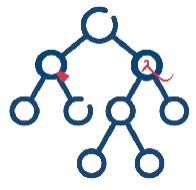
\includegraphics[height=1.0cm]{msca_logo.png}}%
    \end{center}

    \vspace{0.6cm}

    % Main title with Q logos on sides (with clickable links)
    \begin{center}
        \begin{minipage}{0.1\textwidth}
            \centering
            \href{https://quantlet.com}{
\includegraphics[height=1.1cm]{ql_logo.png}}
        \end{minipage}%
        \begin{minipage}{0.78\textwidth}
            \centering
            {\LARGE\bfseries\usebeamercolor[fg]{title}\inserttitle}

            \vspace{0.3cm}

            {\usebeamerfont{subtitle}\usebeamercolor[fg]{title}\insertsubtitle}
        \end{minipage}%
        \begin{minipage}{0.1\textwidth}
            \centering
            \href{https://quantinar.com}{
\includegraphics[height=1.1cm]{qr_logo.png}}
        \end{minipage}
    \end{center}

    \vspace{0.6cm}

    % Authors (left aligned)
    \hspace{0.5cm}{\usebeamerfont{author}\insertauthor}

    \vspace{0.3cm}

    % Institute/Affiliations (left aligned)
    \hspace{0.5cm}\begin{minipage}[t]{0.9\textwidth}
        \raggedright\small\insertinstitute
    \end{minipage}
}

%=============================================================================
% THEOREM ENVIRONMENTS
%=============================================================================
\theoremstyle{definition}
\setbeamertemplate{theorems}[numbered]
\ifdefined\sfmlang
\newtheorem{defn}{Definiție}
\newtheorem{thm}{Teoremă}
\newtheorem{prop}{Propoziție}
\newtheorem{rmk}{Observație}
\else
\newtheorem{defn}{Definition}
\newtheorem{thm}{Theorem}
\newtheorem{prop}{Proposition}
\newtheorem{rmk}{Remark}
\fi

%=============================================================================
% CENTRED MINIPAGE (no extra vertical space)
%=============================================================================
\newenvironment{cminipage}[1]{%
    \par\noindent\hfill\begin{minipage}{#1}\ignorespaces
}{%
    \end{minipage}\hfill\null\par
}

%=============================================================================
% CUSTOM COMMANDS
%=============================================================================
\newcommand{\E}{\mathbb{E}}
\newcommand{\Var}{\text{Var}}
\newcommand{\Cov}{\text{Cov}}
\newcommand{\Corr}{\text{Corr}}
\newcommand{\R}{\mathbb{R}}
\newcommand{\N}{\mathbb{N}}
\newcommand{\Z}{\mathbb{Z}}
\newcommand{\B}{\mathbf{B}}
\newcommand{\imark}{\textcolor{MainBlue}{\textbullet}}
\newcommand{\RMSE}{\text{RMSE}}
\newcommand{\MAE}{\text{MAE}}
\newcommand{\MAPE}{\text{MAPE}}

 se definește
%   \newcommand{\coursename}{Statistics of Financial Markets}      (EN)
%   \newcommand{\coursename}{Statistica piețelor financiare}       (RO)  și  \def\sfmlang{ro}
% Fișierele .tex se află în EN/Courses, EN/Seminars, RO/Cursuri, RO/Seminarii (două niveluri sub rădăcină).
% Deck-urile sînt generate de latex/build_chapterN.py / build_seminarN.py (vezi latex/sfm_build.py).

\documentclass[9pt, aspectratio=169, t]{beamer}
\providecommand{\coursename}{Statistics of Financial Markets}

% Ensure content fits on slides
\setbeamersize{text margin left=8mm, text margin right=8mm}

%=============================================================================
% THEME AND STYLE CONFIGURATION
%=============================================================================
\usetheme{default}
% Using default theme for clean header/footer control

% Color Palette (matching Redispatch PDF)
\definecolor{MainBlue}{RGB}{26, 58, 110}
\definecolor{AccentBlue}{RGB}{26, 58, 110}
\definecolor{IDAred}{RGB}{205, 0, 0}
\definecolor{DarkGray}{RGB}{51, 51, 51}
\definecolor{MediumGray}{RGB}{128, 128, 128}
\definecolor{LightGray}{RGB}{248, 248, 248}
\definecolor{VeryLightGray}{RGB}{235, 235, 235}
\definecolor{KeynoteGray}{RGB}{218, 218, 218}
\definecolor{SectionGray}{RGB}{120, 120, 120}
\definecolor{FooterGray}{RGB}{100, 100, 100}
\definecolor{Crimson}{RGB}{220, 53, 69}
\definecolor{Forest}{RGB}{46, 125, 50}
\definecolor{Amber}{RGB}{181, 133, 63}
\definecolor{Orange}{RGB}{230, 126, 34}
\definecolor{Purple}{RGB}{142, 68, 173}

% Gradient background (exact Keynote 315° gradient: white to RGB 218,218,218)
\setbeamertemplate{background}{%
    \begin{tikzpicture}[remember picture, overlay]
        \shade[shading=axis, shading angle=315,
        top color=white, bottom color=KeynoteGray]
        (current page.south west) rectangle (current page.north east);
    \end{tikzpicture}%
}
% Fallback solid color for compatibility
\setbeamercolor{background canvas}{bg=}

\setbeamercolor{palette primary}{bg=MainBlue, fg=white}
\setbeamercolor{palette secondary}{bg=MainBlue!85, fg=white}
\setbeamercolor{palette tertiary}{bg=MainBlue!70, fg=white}
\setbeamercolor{structure}{fg=MainBlue}
\setbeamercolor{title}{fg=IDAred}
\setbeamercolor{frametitle}{fg=IDAred, bg=}
\setbeamercolor{block title}{bg=MainBlue, fg=white}
\setbeamercolor{block body}{bg=VeryLightGray, fg=DarkGray}
\setbeamercolor{block title alerted}{bg=Crimson, fg=white}
\setbeamercolor{block body alerted}{bg=Crimson!8, fg=DarkGray}
\setbeamercolor{block title example}{bg=Forest, fg=white}
\setbeamercolor{block body example}{bg=Forest!8, fg=DarkGray}
\setbeamercolor{item}{fg=MainBlue}

% Footer colors (override Madrid theme blue)
\setbeamercolor{author in head/foot}{fg=FooterGray, bg=}
\setbeamercolor{title in head/foot}{fg=FooterGray, bg=}
\setbeamercolor{date in head/foot}{fg=FooterGray, bg=}
\setbeamercolor{section in head/foot}{fg=FooterGray, bg=}
\setbeamercolor{subsection in head/foot}{fg=FooterGray, bg=}

% Bullet styles (apply everywhere including blocks)
\setbeamertemplate{itemize item}{\color{MainBlue}$\boxdot$}
\setbeamertemplate{itemize subitem}{\color{MainBlue}$\blacktriangleright$}
\setbeamertemplate{itemize subsubitem}{\color{MainBlue}\tiny$\bullet$}
\setbeamertemplate{itemize/enumerate body begin}{\normalsize}
\setbeamertemplate{itemize/enumerate subbody begin}{\normalsize}

% Item spacing - compact style
\setlength{\leftmargini}{10pt}       % Level 1: minimal indent
\setlength{\leftmarginii}{10pt}      % Level 2: minimal additional indent
% Compact list spacing (zero extra space before/after lists in blocks)
\makeatletter
\def\@listi{\leftmargin\leftmargini \topsep 0pt \parsep 0pt \itemsep 0pt}
\def\@listii{\leftmargin\leftmarginii \topsep 0pt \parsep 0pt \itemsep 0pt}
\makeatother

\setbeamertemplate{navigation symbols}{}

%=============================================================================
% CUSTOM HEADLINE
%=============================================================================
\setbeamertemplate{headline}{%
    \vskip10pt%
    \hbox to \paperwidth{%
        \hskip0.5cm%
        {\small\color{FooterGray}\renewcommand{\hyperlink}[2]{##2}\insertsectionhead}%
        \hfill%
        \textcolor{FooterGray}{\small\insertframenumber}%
        \hskip0.5cm%
    }%
    \vskip4pt%
    {\color{FooterGray}\hrule height 0.4pt}%
}

%=============================================================================
% CUSTOM FOOTER
%=============================================================================
\usepackage{fontawesome5}

\setbeamertemplate{footline}{%
    {\color{FooterGray}\hrule height 0.4pt}%
    \vskip4pt%
    \hbox to \paperwidth{%
        \hskip0.5cm%
        \textcolor{FooterGray}{\small\coursename}%
        \hfill%
        \raisebox{-0.1em}{%
            \begin{tikzpicture}[x=0.08em, y=0.08em, line width=0.4pt]
                \draw[FooterGray] (0,3) -- (1,4) -- (2,3.5) -- (3,5) -- (4,4) -- (5,6) -- (6,5.5) -- (7,4) -- (8,5) -- (9,7) -- (10,6) -- (11,5) -- (12,6.5) -- (13,8) -- (14,7) -- (15,6) -- (16,7.5) -- (17,9) -- (18,8) -- (19,7) -- (20,8.5) -- (21,10) -- (22,9) -- (23,8) -- (24,9.5);
            \end{tikzpicture}%
        }%
        \hskip0.5cm%
    }%
    \vskip6pt%
}

%=============================================================================
% PACKAGES
%=============================================================================
\usepackage[utf8]{inputenc}
\DeclareUnicodeCharacter{03B1}{\ensuremath{\alpha}}
\usepackage[T1]{fontenc}
\usepackage{amsmath, amssymb, amsthm}
\usepackage{mathtools}
\usepackage{bm}
\usepackage{tikz}
\usetikzlibrary{arrows.meta, positioning, shapes, calc, decorations.pathreplacing, shadings}
\usepackage{booktabs}
\usepackage{multirow}
\usepackage{array}
\usepackage{graphicx}
\usepackage{hyperref}
\usepackage{colortbl}
\usepackage{listings}
\lstset{language=Python, basicstyle=\ttfamily\scriptsize, keywordstyle=\color{MainBlue}\bfseries,
  commentstyle=\color{Forest}, stringstyle=\color{Crimson}, breaklines=true,
  frame=none, backgroundcolor=\color{VeryLightGray}, xleftmargin=2mm}
\hypersetup{colorlinks=true, linkcolor=MainBlue, urlcolor=MainBlue}
\graphicspath{{../../logos/}{../../charts/}{../../photos/}}
\usepackage{xcolor}
\hfuzz=2pt  % Suppress tiny overfull warnings (<2pt)
\vfuzz=2pt  % Suppress tiny vertical overfull warnings (<2pt)

%=============================================================================
% QUANTLET COMMANDS
%   \quantlet{<displayed name>}{<url>}       (generic, compatible with the older SFM decks)
%   \sfmquantlet{Ch_05}{SFM_ch5_garch}       -> https://github.com/danpele/SFM/tree/main/Quantlets/Ch_05/SFM_ch5_garch
%   \qlurl{<folder>} is defined per chapter by the generator (Quantlets/Ch_NN/<folder>)
%=============================================================================
\newcommand{\sfmrepo}{https://github.com/danpele/SFM}
\newcommand{\sfmqlbase}{https://github.com/danpele/SFM/tree/main/Quantlets}
\newcommand{\quantlet}[2]{%
    \hfill\href{#2}{%
        \raisebox{-0.15em}{
\includegraphics[height=0.7em]{ql_logo.png}}%
        \textcolor{MainBlue}{\tiny\ #1}%
    }%
}
\newcommand{\sfmquantlet}[2]{\quantlet{\detokenize{#2}}{\sfmqlbase/#1/#2}}

%=============================================================================
% NOTEBOOKS (Google Colab)
%   \colaburl{notebooks/EN/chapter5_seminar_notebook.ipynb} -> the Colab link of a file in the SFM repo
%   \nb: the chapter notebook (each seminar deck redefines it with \renewcommand)
%=============================================================================
\newcommand{\colaburl}[1]{https://colab.research.google.com/github/danpele/SFM/blob/main/#1}
\newcommand{\nb}{https://colab.research.google.com/github/danpele/SFM/tree/main/notebooks/EN}
\newcommand{\nbname}{notebooks/EN}

%=============================================================================
% SLIDE HELPERS (used by the generators; the same as in MFM)
%=============================================================================
% local font size for list bodies (the preamble forces \normalsize)
\newcommand{\itemsize}[1]{\setbeamertemplate{itemize/enumerate body begin}{#1}\setbeamertemplate{itemize/enumerate subbody begin}{#1}}
\newcommand{\intitle}[1]{{\hypersetup{urlcolor=white}#1}}   % white links inside coloured title bars
\newcommand{\imgcap}[1]{{\scriptsize #1}\\[0.5mm]}          % caption under a photo
\newcommand{\imgcredit}[2]{{\tiny\color{FooterGray}\href{#1}{#2}}}   % image credit: source URL, author/licence
\newcommand{\aiprompt}[1]{{\ttfamily\color{MainBlue}#1}}     % a prompt to an AI assistant

%=============================================================================
% SEMINARS: student version by default; the instructor wrapper *_solutions.tex sets \solutionstrue
%=============================================================================
\makeatletter\@ifundefined{ifsolutions}{\expandafter\newif\csname ifsolutions\endcsname}{}\makeatother
\newcommand{\solonly}[1]{\ifsolutions #1\fi}
\newcommand{\propsub}{\ifsolutions\else\framesubtitle{\ifdefined\sfmlang Rezolvarea se discută la seminar\else Solution discussed in class\fi}\fi}

%=============================================================================
% APPENDIX AND CHAPTER LINKS (latex/appendix_links.py writes the calls; it also re-declares these
% macros before \begin{document}, so the decks compile with or without this preamble block)
%=============================================================================
\providecommand{\sfmapplink}[3]{\hypertarget{#2}{}\hyperlink{#1}{\beamergotobutton{#3}}}
\providecommand{\sfmappback}[2]{\begin{tikzpicture}[remember picture,overlay]\node[anchor=south east] at ([xshift=-3mm,yshift=7mm]current page.south east){\hyperlink{#1}{\beamerreturnbutton{#2}}};\end{tikzpicture}}
\providecommand{\sfmchlink}[2]{\href{#1}{#2}}
\providecommand{\sfmchlinkt}[2]{\href{#1}{\usebeamercolor[fg]{frametitle}#2}}

%=============================================================================
% QUANTINAR COMMAND: link către un curs Quantinar (subiecte avansate)
%=============================================================================
\newcommand{\quantinar}[2]{%
    \href{#2}{%
        \raisebox{-0.15em}{
\includegraphics[height=0.8em]{qr_logo.png}}%
        \textcolor{MainBlue}{\scriptsize\ #1}%
    }%
}

%=============================================================================
% CUSTOM TITLE PAGE
%=============================================================================
\defbeamertemplate*{title page}{hybrid}[1][]
{
    \vspace{0.2cm}
    % Logos row - top header (with clickable links)
    \begin{center}
        \href{https://www.ase.ro}{
\includegraphics[height=1.0cm]{ase_logo.png}}\hspace{0.3cm}%
        \href{https://theida.net}{
\includegraphics[height=1.0cm]{ida_logo.png}}\hspace{0.3cm}%
        \href{https://blockchain-research-center.com}{
\includegraphics[height=1.0cm]{brc_logo.png}}\hspace{0.3cm}%
        \href{https://www.ai4efin.ase.ro}{
\includegraphics[height=1.0cm]{ai4efin_logo.png}}\hspace{0.3cm}%
        \href{https://ipe.ro/new}{
\includegraphics[height=1.0cm]{acad_logo.png}}\hspace{0.3cm}%
        \href{https://www.digital-finance-msca.com}{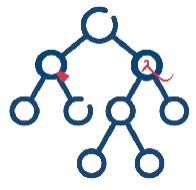
\includegraphics[height=1.0cm]{msca_logo.png}}%
    \end{center}

    \vspace{0.6cm}

    % Main title with Q logos on sides (with clickable links)
    \begin{center}
        \begin{minipage}{0.1\textwidth}
            \centering
            \href{https://quantlet.com}{
\includegraphics[height=1.1cm]{ql_logo.png}}
        \end{minipage}%
        \begin{minipage}{0.78\textwidth}
            \centering
            {\LARGE\bfseries\usebeamercolor[fg]{title}\inserttitle}

            \vspace{0.3cm}

            {\usebeamerfont{subtitle}\usebeamercolor[fg]{title}\insertsubtitle}
        \end{minipage}%
        \begin{minipage}{0.1\textwidth}
            \centering
            \href{https://quantinar.com}{
\includegraphics[height=1.1cm]{qr_logo.png}}
        \end{minipage}
    \end{center}

    \vspace{0.6cm}

    % Authors (left aligned)
    \hspace{0.5cm}{\usebeamerfont{author}\insertauthor}

    \vspace{0.3cm}

    % Institute/Affiliations (left aligned)
    \hspace{0.5cm}\begin{minipage}[t]{0.9\textwidth}
        \raggedright\small\insertinstitute
    \end{minipage}
}

%=============================================================================
% THEOREM ENVIRONMENTS
%=============================================================================
\theoremstyle{definition}
\setbeamertemplate{theorems}[numbered]
\ifdefined\sfmlang
\newtheorem{defn}{Definiție}
\newtheorem{thm}{Teoremă}
\newtheorem{prop}{Propoziție}
\newtheorem{rmk}{Observație}
\else
\newtheorem{defn}{Definition}
\newtheorem{thm}{Theorem}
\newtheorem{prop}{Proposition}
\newtheorem{rmk}{Remark}
\fi

%=============================================================================
% CENTRED MINIPAGE (no extra vertical space)
%=============================================================================
\newenvironment{cminipage}[1]{%
    \par\noindent\hfill\begin{minipage}{#1}\ignorespaces
}{%
    \end{minipage}\hfill\null\par
}

%=============================================================================
% CUSTOM COMMANDS
%=============================================================================
\newcommand{\E}{\mathbb{E}}
\newcommand{\Var}{\text{Var}}
\newcommand{\Cov}{\text{Cov}}
\newcommand{\Corr}{\text{Corr}}
\newcommand{\R}{\mathbb{R}}
\newcommand{\N}{\mathbb{N}}
\newcommand{\Z}{\mathbb{Z}}
\newcommand{\B}{\mathbf{B}}
\newcommand{\imark}{\textcolor{MainBlue}{\textbullet}}
\newcommand{\RMSE}{\text{RMSE}}
\newcommand{\MAE}{\text{MAE}}
\newcommand{\MAPE}{\text{MAPE}}



\newcommand{\qlurl}[1]{https://github.com/danpele/SFM/tree/main/Quantlets/Ch_16/#1}

% Clickable citations (DOIs verified via Crossref)

\newcommand{\refFHH}{\href{https://doi.org/10.1007/978-3-030-13751-9}{Franke, Härdle \& Hafner (2019)}}
\newcommand{\refBHL}{\href{https://doi.org/10.1007/978-3-642-33929-5}{Borak, Härdle \& López-Cabrera (2013)}}
\newcommand{\refTsay}{\href{https://doi.org/10.1002/9780470644560}{Tsay (2010)}}
\newcommand{\refCLM}{\href{https://doi.org/10.1515/9781400830213}{Campbell, Lo \& MacKinlay (1997)}}
\newcommand{\refQRM}{\href{https://press.princeton.edu/books/hardcover/9780691166278/quantitative-risk-management}{McNeil, Frey \& Embrechts (2015)}}
\newcommand{\refCont}{\href{https://doi.org/10.1080/713665670}{Cont (2001)}}
\newcommand{\refMandelbrot}{\href{https://doi.org/10.1086/294632}{Mandelbrot (1963)}}
\newcommand{\refNolan}{\href{https://doi.org/10.1007/978-3-030-52915-4}{Nolan (2020)}}
\newcommand{\refJB}{\href{https://doi.org/10.1016/0165-1765(80)90024-5}{Jarque \& Bera (1980)}}
\newcommand{\refHill}{\href{https://doi.org/10.1214/aos/1176343247}{Hill (1975)}}
\newcommand{\refFama}{\href{https://doi.org/10.2307/2325486}{Fama (1970)}}
\newcommand{\refLM}{\href{https://doi.org/10.1093/rfs/1.1.41}{Lo \& MacKinlay (1988)}}
\newcommand{\refEngle}{\href{https://doi.org/10.2307/1912773}{Engle (1982)}}
\newcommand{\refBoll}{\href{https://doi.org/10.1016/0304-4076(86)90063-1}{Bollerslev (1986)}}
\newcommand{\refRM}{\href{https://www.msci.com/documents/10199/5915b101-4206-4ba0-aee2-3449d5c7e95a}{J.P.\ Morgan/Reuters (1996)}}
\newcommand{\refArtzner}{\href{https://doi.org/10.1111/1467-9965.00068}{Artzner et al.\ (1999)}}
\newcommand{\refKupiec}{\href{https://doi.org/10.3905/jod.1995.407942}{Kupiec (1995)}}
\newcommand{\refHurst}{\href{https://doi.org/10.1061/TACEAT.0006518}{Hurst (1951)}}
\newcommand{\refPeters}{\href{https://www.wiley.com/en-us/Fractal+Market+Analysis\%3A+Applying+Chaos+Theory+to+Investment+and+Economics-p-9780471585244}{Peters (1994)}}
\newcommand{\refAltman}{\href{https://doi.org/10.1111/j.1540-6261.1968.tb00843.x}{Altman (1968)}}
\newcommand{\refGKX}{\href{https://doi.org/10.1093/rfs/hhaa009}{Gu, Kelly \& Xiu (2020)}}
\newcommand{\refNakamoto}{\href{https://bitcoin.org/bitcoin.pdf}{Nakamoto (2008)}}
\newcommand{\refAB}{\href{https://doi.org/10.1257/aer.20120555}{Adrian \& Brunnermeier (2016)}}
\newcommand{\refDY}{\href{https://doi.org/10.1016/j.ijforecast.2011.02.006}{Diebold \& Yilmaz (2012)}}
\newcommand{\refMenk}{\href{https://doi.org/10.1111/jofi.13337}{Menkveld et al.\ (2024)}}
\newcommand{\refWang}{\href{https://doi.org/10.1038/s41586-023-06221-2}{Wang et al.\ (2023)}}

\title[Statistics of Financial Markets]{Statistics of Financial Markets}
\subtitle{Chapter 16: Review}
\author[D.T. Pele]{Daniel Traian PELE}
\institute{Bucharest University of Economic Studies\\
IDA Institute Digital Assets\\
Blockchain Research Center\\
AI4EFin Artificial Intelligence for Energy Finance\\
Romanian Academy, Institute for Economic Forecasting\\
MSCA Digital Finance}
\date{}

%=============================================================================
\providecommand{\sfmapplink}[3]{\hypertarget{#2}{}\hyperlink{#1}{\beamergotobutton{#3}}}  % APPLINKS-MACROS
\providecommand{\sfmappback}[2]{\begin{tikzpicture}[remember picture,overlay]\node[anchor=south east] at ([xshift=-3mm,yshift=7mm]current page.south east){\hyperlink{#1}{\beamerreturnbutton{#2}}};\end{tikzpicture}}  % APPLINKS-MACROS
\providecommand{\sfmchlink}[2]{\href{#1}{#2}}  % APPLINKS-MACROS
\providecommand{\sfmchlinkt}[2]{\href{#1}{\usebeamercolor[fg]{frametitle}#2}}  % APPLINKS-MACROS
\begin{document}
%=============================================================================

{
\setbeamertemplate{headline}{}
\setbeamertemplate{footline}{}
\begin{frame}[noframenumbering]
    \titlepage
\end{frame}
}
% BEGIN-ACRONYMS (generat de latex/acronyms.py; nu editati manual)
\begin{frame}{Acronyms used in this material (1/2)}
\setbeamertemplate{itemize/enumerate body begin}{\tiny}
\begin{columns}[T]
\begin{column}{0.49\textwidth}
\begin{itemize}\setlength{\itemsep}{0pt}
    \item \textbf{ACF}: Autocorrelation Function
    \item \textbf{AD}: Anderson–Darling (test)
    \item \textbf{AI}: Artificial Intelligence
    \item \textbf{AIC}: Akaike Information Criterion
    \item \textbf{ARCH}: AutoRegressive Conditional Heteroskedasticity
    \item \textbf{ARCH-LM}: ARCH Lagrange Multiplier (test)
    \item \textbf{AUC}: Area Under the (ROC) Curve
    \item \textbf{BET}: Bucharest Exchange Trading (index)
    \item \textbf{BIC}: Bayesian Information Criterion
    \item \textbf{CAGR}: Compound Annual Growth Rate
    \item \textbf{CDF}: Cumulative Distribution Function
    \item \textbf{CI}: Confidence Interval
    \item \textbf{DFA}: Detrended Fluctuation Analysis
\end{itemize}
\end{column}
\begin{column}{0.49\textwidth}
\begin{itemize}\setlength{\itemsep}{0pt}
    \item \textbf{EAD}: Exposure At Default
    \item \textbf{EGARCH}: Exponential GARCH
    \item \textbf{EODHD}: EOD Historical Data (market-data provider)
    \item \textbf{ES}: Expected Shortfall
    \item \textbf{EVT}: Extreme Value Theory
    \item \textbf{EWMA}: Exponentially Weighted Moving Average
    \item \textbf{FHS}: Filtered Historical Simulation
    \item \textbf{FPR}: False Positive Rate
    \item \textbf{GARCH}: Generalised AutoRegressive Conditional Heteroskedasticity
    \item \textbf{GBM}: Geometric Brownian Motion
    \item \textbf{GEV}: Generalised Extreme Value (distribution)
    \item \textbf{GJR}: Glosten–Jagannathan–Runkle (asymmetric GARCH)
    \item \textbf{GPD}: Generalised Pareto Distribution
\end{itemize}
\end{column}
\end{columns}
\end{frame}
\begin{frame}{Acronyms used in this material (2/2)}
\setbeamertemplate{itemize/enumerate body begin}{\tiny}
\begin{columns}[T]
\begin{column}{0.49\textwidth}
\begin{itemize}\setlength{\itemsep}{0pt}
    \item \textbf{GPH}: Geweke–Porter-Hudak (log-periodogram estimator)
    \item \textbf{HAR}: Heterogeneous AutoRegressive (model)
    \item \textbf{HS}: Historical Simulation
    \item \textbf{IGARCH}: Integrated GARCH
    \item \textbf{JB}: Jarque–Bera (test)
    \item \textbf{KS}: Kolmogorov–Smirnov (test)
    \item \textbf{LDA}: Linear Discriminant Analysis
    \item \textbf{LGD}: Loss Given Default
    \item \textbf{LR}: Likelihood Ratio
    \item \textbf{MDD}: Maximum DrawDown
    \item \textbf{MES}: Marginal Expected Shortfall
    \item \textbf{NIG}: Normal Inverse Gaussian (distribution)
    \item \textbf{PD}: Probability of Default
\end{itemize}
\end{column}
\begin{column}{0.49\textwidth}
\begin{itemize}\setlength{\itemsep}{0pt}
    \item \textbf{QLIKE}: Quasi-LIKElihood (loss function)
    \item \textbf{QQ}: Quantile–Quantile (plot)
    \item \textbf{SE}: Standard Error
    \item \textbf{SR}: Sharpe Ratio
    \item \textbf{SRISK}: Systemic RISK (capital shortfall in a crisis)
    \item \textbf{TPR}: True Positive Rate
    \item \textbf{US}: United States
    \item \textbf{VR}: Variance Ratio
\end{itemize}
\end{column}
\end{columns}
\end{frame}
% END-ACRONYMS

\begin{frame}{Today's Question and Route}
\itemsize{\small}
\begin{columns}[T]
\begin{column}{0.58\textwidth}
\begin{itemize}
    \item \textbf{Question}: what does the whole course say about the returns of the BET, the S\&P 500 and Bitcoin, and how is it examined?
    \begin{itemize}
        \item one chapter that ties \sfmchlink{https://danpele.github.io/SFM/EN/Courses/chapter0_introduction.pdf}{Chapters 0}--\sfmchlink{https://danpele.github.io/SFM/EN/Courses/chapter15_systemic_risk.pdf}{15} together
    \end{itemize}
    \item \textbf{Route}
    \begin{itemize}
        \item Part I: the course map, two recap slides per chapter, the toolbox of tests and models
        \item Part II: the exam (format, grading, eight solved problems) and the team project
        \item Part III: how AI could help in your own research
    \end{itemize}
\end{itemize}
\end{column}
\begin{column}{0.38\textwidth}
\centering
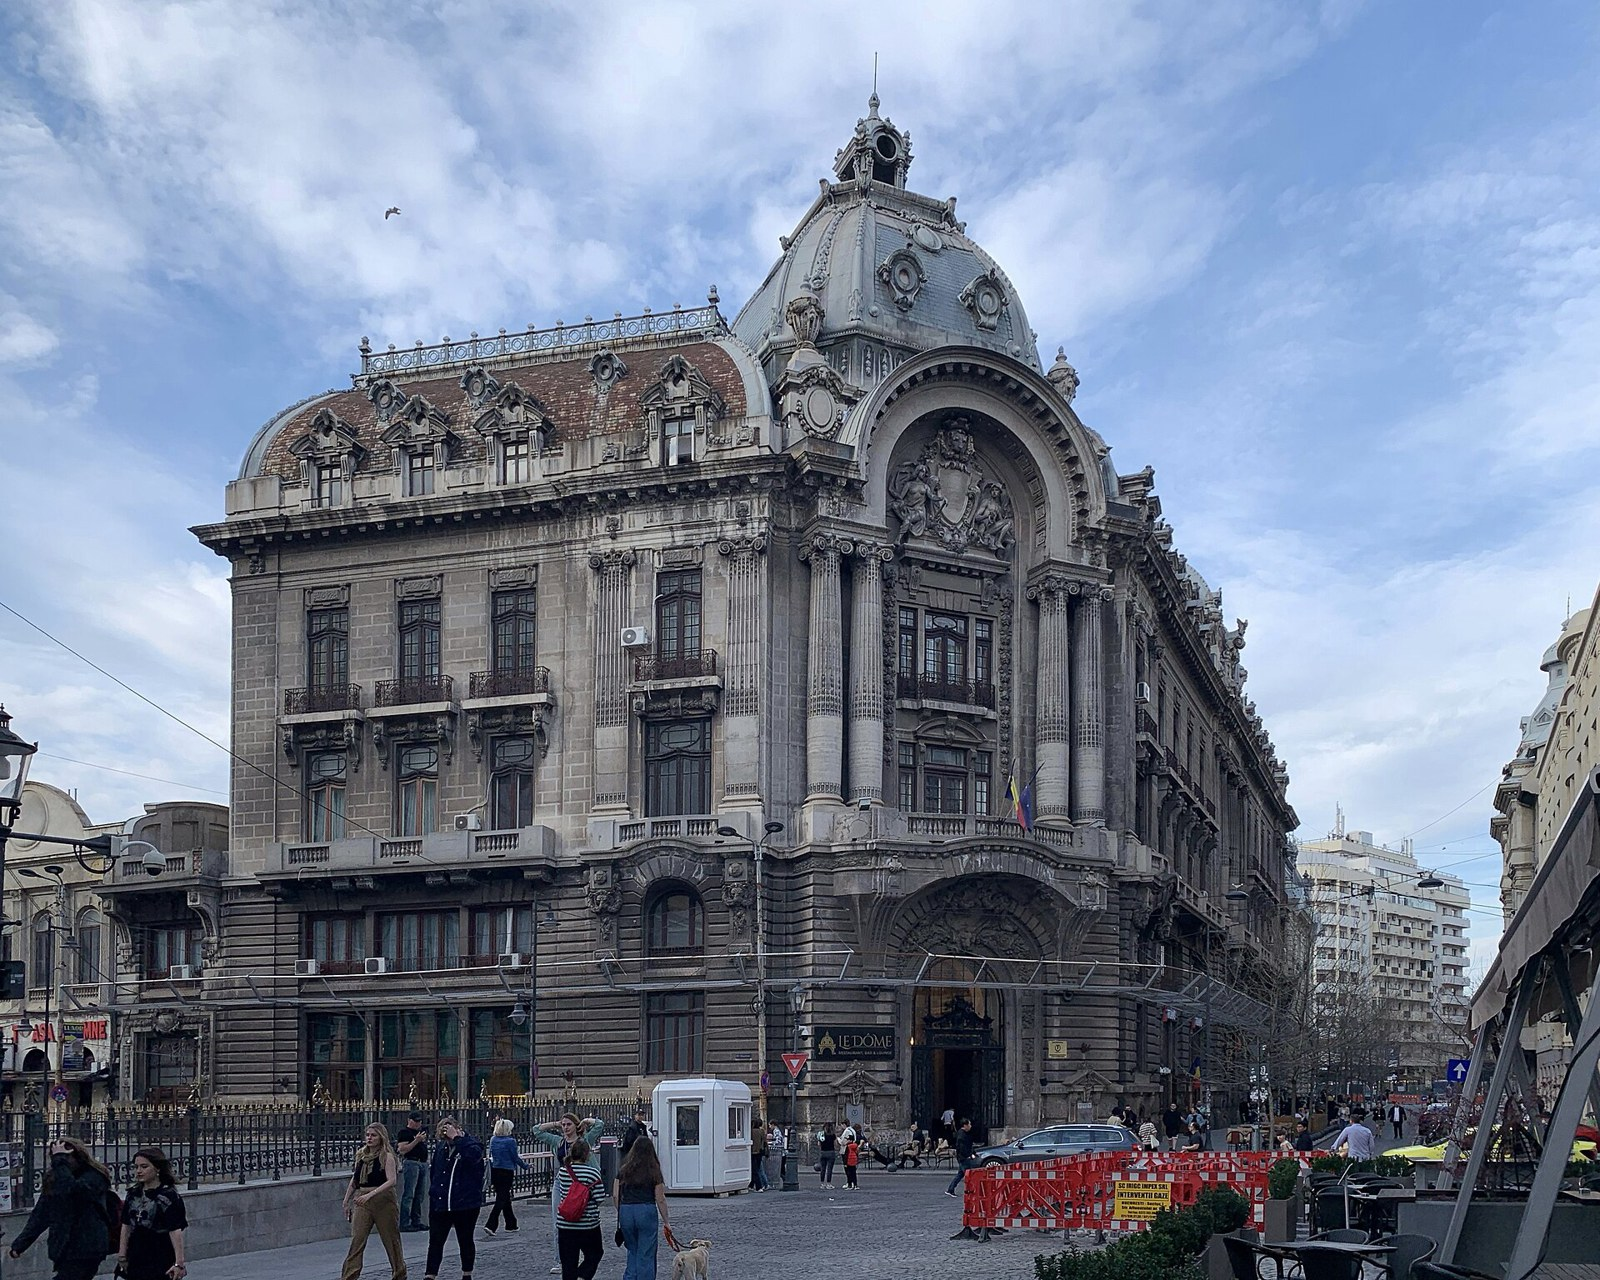
\includegraphics[height=0.40\textheight]{ch0_bvb_palace_2023.jpg}\\[1mm]
\imgcap{The Stock Exchange Palace, Bucharest}
\imgcredit{https://commons.wikimedia.org/wiki/File:Bucure\%C8\%99ti_-_Palatul_Bursei_(2023)_-_img_01.jpg}{Photo: Chainwit.\ (2023); CC BY 4.0; Wikimedia Commons}
\end{column}
\end{columns}
\end{frame}

\begin{frame}{Learning Outcomes}
\itemsize{\small}
\begin{itemize}
    \item Place every chapter on the path from prices to risk numbers and name the question it answers
    \item Recall the key formula, the key empirical fact and the most common mistake of each chapter
    \item Choose the right test or model for a given question about a return series
    \item Solve exam-type problems step by step and interpret the result in three to five sentences
    \item Plan the team project, its oral defence and the declaration of AI use
\end{itemize}
\end{frame}

\begin{frame}{Reading and Tools}
\itemsize{\small}
\begin{itemize}
    \item Textbook: \refFHH; exercises with solutions: \refBHL
    \begin{itemize}
        \item time series and volatility: \refTsay; market efficiency: \refCLM; risk measures: \refQRM
    \end{itemize}
    \item Python Quantlets of this chapter: \href{https://github.com/danpele/SFM/tree/main/Quantlets/Ch_16}{Quantlets/Ch\_16}
    \begin{itemize}
        \item the course in one table: S\&P 500, BET and Bitcoin on one common window
    \end{itemize}
    \item Lecture notebook, the course in one notebook: \href{\colaburl{notebooks/EN/chapter16_lecture_notebook.ipynb}}{open in Google Colab}
    \item Video course: \quantinar{Statistics of Financial Markets}{https://quantinar.com/course/103/statistics-of-financial-markets}
    \item Self-assessment: the quiz of this chapter, 20 questions from all chapters
\end{itemize}
\end{frame}


%=============================================================================
\section{The Course Map}
%=============================================================================

\begin{frame}{The Course Map: \sfmchlinkt{https://danpele.github.io/SFM/EN/Courses/chapter0_introduction.pdf}{Chapters 0}--\sfmchlinkt{https://danpele.github.io/SFM/EN/Courses/chapter15_systemic_risk.pdf}{15}}
\itemsize{\footnotesize}
\begin{center}
\resizebox{0.97\textwidth}{!}{%
\begin{tikzpicture}[
  box/.style={draw=MainBlue, rounded corners=2pt, fill=white, font=\scriptsize, align=center, minimum width=2.2cm, minimum height=0.85cm, text width=2.1cm},
  key/.style={box, draw=IDAred, line width=0.9pt},
  lab/.style={font=\scriptsize\bfseries, text=MainBlue, anchor=east, align=right},
  arr/.style={-{Stealth[length=2mm]}, MainBlue, line width=0.5pt},
  karr/.style={-{Stealth[length=2.4mm]}, IDAred, line width=1.1pt}]
\node[lab] at (-0.1, 0) {Data and\\ distributions};
\node[box] (c0) at (1.3, 0) {0 Markets\\ and data};
\node[key] (c1) at (3.8, 0) {1 Returns,\\ indicators};
\node[key] (c2) at (6.3, 0) {2 Distributions,\\ stylised facts};
\node[box] (c3) at (8.8, 0) {3 $\alpha$-stable\\ laws};
\node[key] (c5) at (11.3, 0) {5 Heavy tails,\\ EVT};
\node[box] (c6) at (13.8, 0) {6 Model\\ selection};
\node[lab] at (-0.1, -1.7) {Time, volatility\\ and risk};
\node[box] (c4) at (1.3, -1.7) {4 Probability,\\ processes};
\node[box] (c7) at (3.8, -1.7) {7 Efficiency,\\ VR tests};
\node[box] (c11) at (6.3, -1.7) {11 Long\\ memory};
\node[box] (c8) at (8.8, -1.7) {8 Volatility\\ estimators};
\node[key] (c9) at (11.3, -1.7) {9 ARCH, GARCH};
\node[key] (c10) at (13.8, -1.7) {10 VaR, ES,\\ backtesting};
\node[lab] at (-0.1, -3.4) {Applications};
\node[box] (c12) at (6.3, -3.4) {12 Scoring\\ models};
\node[box] (c13) at (8.8, -3.4) {13 Machine\\ learning};
\node[box] (c14) at (11.3, -3.4) {14 Crypto\\ assets};
\node[box] (c15) at (13.8, -3.4) {15 Systemic\\ risk};
\draw[arr] (c0) -- (c1); \draw[karr] (c1) -- (c2); \draw[arr] (c2) -- (c3); \draw[arr] (c3) -- (c5); \draw[arr] (c5) -- (c6);
\draw[karr] (c2.south east) -- (c8.north west); \draw[karr] (c5) -- (c10.north west); \draw[arr] (c6) -- (c10);
\draw[arr] (c4) -- (c7); \draw[arr] (c7) -- (c11); \draw[arr] (c11) -- (c8); \draw[karr] (c8) -- (c9); \draw[karr] (c9) -- (c10);
\draw[arr] (c1) -- (c7); \draw[arr] (c4.south) -- (1.3, -2.6) -- (6.3, -2.6) -- (c12.north);
\draw[arr] (c10) -- (c15); \draw[arr] (c10.south west) -- (c14.north east); \draw[arr] (c9.south west) -- (c13.north east);
\end{tikzpicture}}
\end{center}
\vspace{-0.2cm}
\begin{itemize}
    \item Red: the main thread, from returns and their distribution to a risk number we can test (\sfmchlink{https://danpele.github.io/SFM/EN/Courses/chapter10_var_es_backtesting.pdf}{Chapter 10})
    \item Row 2: dependence in time; the sign of returns is hard to predict (\sfmchlink{https://danpele.github.io/SFM/EN/Courses/chapter7_efficient_markets_random_walk_vr.pdf}{Chapters 7}, \sfmchlink{https://danpele.github.io/SFM/EN/Courses/chapter11_fractal_markets_long_memory.pdf}{11}), their size is predictable (\sfmchlink{https://danpele.github.io/SFM/EN/Courses/chapter8_volatility_estimators.pdf}{Chapters 8}--\sfmchlink{https://danpele.github.io/SFM/EN/Courses/chapter9_arch_garch_models.pdf}{9})
    \item Row 3: the same tools applied to credit, prediction, crypto assets and the banking system
\end{itemize}
\end{frame}

\begin{frame}{The Main Thread: From Prices to Decisions}
\itemsize{\small}
\begin{itemize}
    \item \textbf{Data} (\sfmchlink{https://danpele.github.io/SFM/EN/Courses/chapter0_introduction.pdf}{Chapters 0}--\sfmchlink{https://danpele.github.io/SFM/EN/Courses/chapter1_data_returns_indicators.pdf}{1}): prices from one source, adjusted, on the right calendar
    \begin{itemize}
        \item returns: $r_t = \ln(P_t/P_{t-1})$, in \% for one day
    \end{itemize}
    \item \textbf{Distribution} (\sfmchlink{https://danpele.github.io/SFM/EN/Courses/chapter2_classical_distributions_stylised_facts.pdf}{Chapters 2}--\sfmchlink{https://danpele.github.io/SFM/EN/Courses/chapter6_model_selection_risk_management.pdf}{6}): heavy tails, not the Normal distribution
    \begin{itemize}
        \item Student-$t$, stable laws, EVT; the model is chosen with likelihood, AIC and tail tests
    \end{itemize}
    \item \textbf{Dependence in time} (\sfmchlink{https://danpele.github.io/SFM/EN/Courses/chapter7_efficient_markets_random_walk_vr.pdf}{Chapters 7}--\sfmchlink{https://danpele.github.io/SFM/EN/Courses/chapter11_fractal_markets_long_memory.pdf}{11}): the sign is almost unpredictable, the size is predictable
    \begin{itemize}
        \item variance ratio and Hurst for the mean; EWMA and GARCH for the variance
    \end{itemize}
    \item \textbf{Risk} (\sfmchlink{https://danpele.github.io/SFM/EN/Courses/chapter10_var_es_backtesting.pdf}{Chapter 10}): VaR 1\% and ES 2.5\%, with a backtest
    \begin{itemize}
        \item the applications (\sfmchlink{https://danpele.github.io/SFM/EN/Courses/chapter12_scoring_models.pdf}{Chapters 12}--\sfmchlink{https://danpele.github.io/SFM/EN/Courses/chapter15_systemic_risk.pdf}{15}) reuse the same chain: data, distribution, dependence, risk, evaluation
    \end{itemize}
\end{itemize}
\end{frame}

\begin{frame}{Three Series, One Window: S\&P 500, BET, Bitcoin}
\itemsize{\footnotesize}
\begin{center}
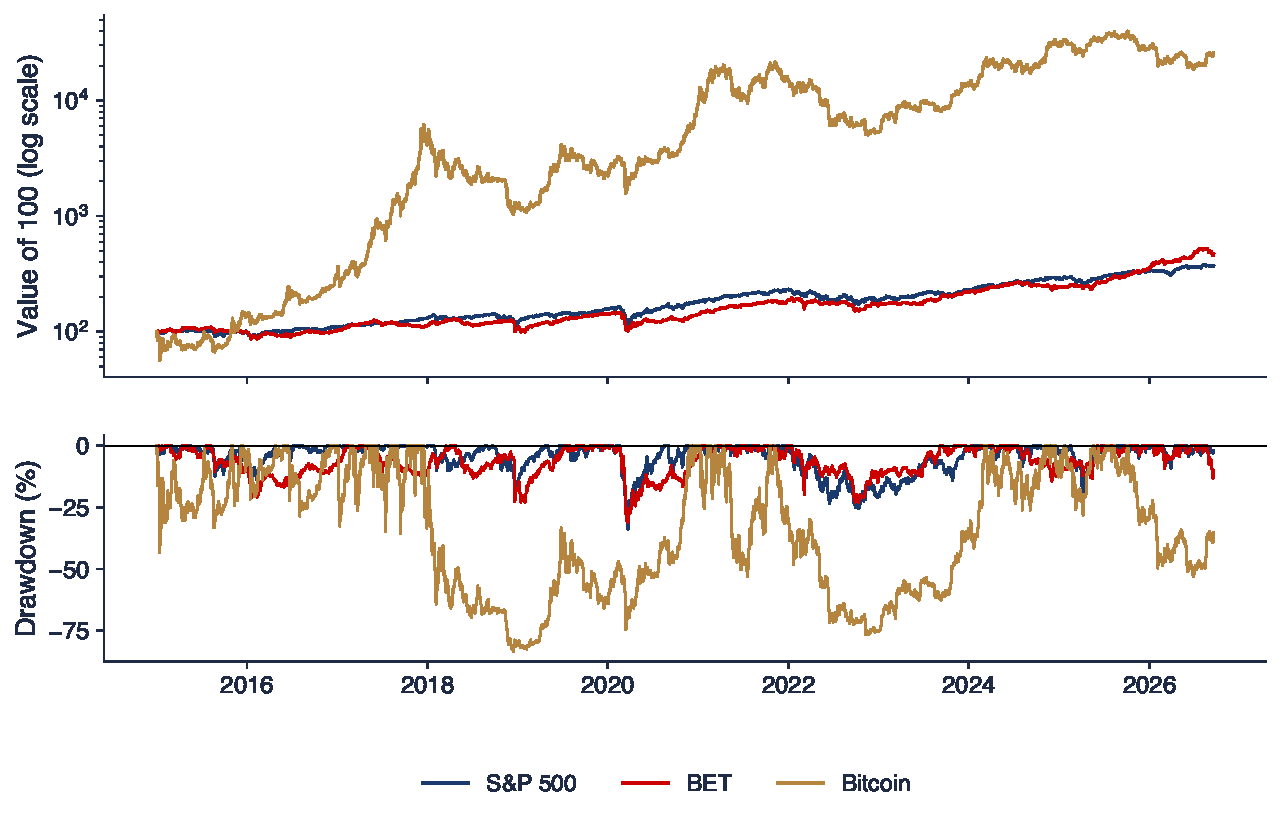
\includegraphics[width=0.97\textwidth,height=0.55\textheight,keepaspectratio]{sfm_ch16_three_series.pdf}
\end{center}
\vspace{-0.25cm}
\begin{itemize}
    \item 100 invested on 2 January 2015 (log scale) and the drawdown $P_t/\max_{s \le t}P_s - 1$
    \item Maximum drawdown: S\&P 500 $-33.9\%$, BET $-31.1\%$ (both in March 2020), Bitcoin $-83.4\%$
\end{itemize}
\sfmquantlet{Ch_16}{SFM_ch16_course_summary}
\end{frame}

\begin{frame}{The Course in One Table}
\itemsize{\footnotesize}
\begin{center}
\scriptsize
\begin{tabular}{lrrr}
\toprule
\textbf{Daily log returns} & S\&P 500 & BET & Bitcoin \\
\midrule
Observations (per year) & 2\,943 (252) & 2\,925 (250) & 4\,278 (365) \\
Mean log return, \% a year & $11.2$ & $13.2$ & $47.4$ \\
Volatility, \% a year & $17.7$ & $15.5$ & $66.7$ \\
Sharpe ratio ($r_f = 0$) $\pm$ SE & $0.72 \pm 0.33$ & $0.93 \pm 0.35$ & $1.04 \pm 0.36$ \\
Skewness; excess kurtosis & $-0.64$; $15.8$ & $-1.41$; $17.8$ & $-0.73$; $12.2$ \\
Hill tail index of losses ($k = 2.5\%\,n$) & $2.75$ & $2.19$ & $2.67$ \\
Ljung--Box $Q(10)$: $r_t$; $r_t^2$ & $236$; $3166$ & $55$; $701$ & $21$; $211$ \\
VR(5); robust $Z^*(5)$ & $0.84$; $-1.34$ & $1.17$; $1.93$ & $0.99$; $-0.22$ \\
GARCH(1,1)-$t$: $\alpha + \beta$ & $0.993$ & $0.925$ & $1.000$ \\
VaR 1\%: historical; Normal (\%) & $3.29$; $2.55$ & $2.72$; $2.23$ & $10.60$; $7.99$ \\
ES 2.5\%, historical (\%) & $3.53$ & $3.21$ & $10.93$ \\
Hurst (R/S): $r_t$; $|r_t|$ & $0.53$; $0.84$ & $0.59$; $0.75$ & $0.59$; $0.78$ \\
\bottomrule
\end{tabular}
\end{center}
\begin{itemize}
    \item Window: 5 January 2015 -- 18 September 2026; each series on its own calendar (Bitcoin: 365 days a year); critical value of $\chi^2(10)$ at 5\%: $18.31$
\end{itemize}\sfmquantlet{Ch_16}{SFM_ch16_course_summary}
\end{frame}

\begin{frame}{Interpreting the Table}
\itemsize{\small}
\begin{itemize}
    \item \textbf{Return and risk}: Bitcoin has about four times the volatility of the two indices
    \begin{itemize}
        \item the Sharpe ratios are close once their standard errors are taken into account
    \end{itemize}
    \item \textbf{Distribution}: negative skewness, excess kurtosis above 10, Hill indices between 2 and 3
    \begin{itemize}
        \item the Normal VaR 1\% is too low by 22\% (S\&P 500), 18\% (BET) and 25\% (Bitcoin)
    \end{itemize}
    \item \textbf{Dependence}: Ljung--Box on $r_t^2$ is many times larger than on $r_t$
    \begin{itemize}
        \item the robust VR test rejects no random walk at 5\% here; $H$ of $|r_t|$ is far above 0.5
        \item volatility is persistent: $\alpha + \beta$ close to 1 (Bitcoin: an IGARCH, $\alpha + \beta = 1$)
    \end{itemize}
\end{itemize}
\end{frame}

\begin{frame}{Stylised Facts in One Chart}
\itemsize{\footnotesize}
\begin{center}
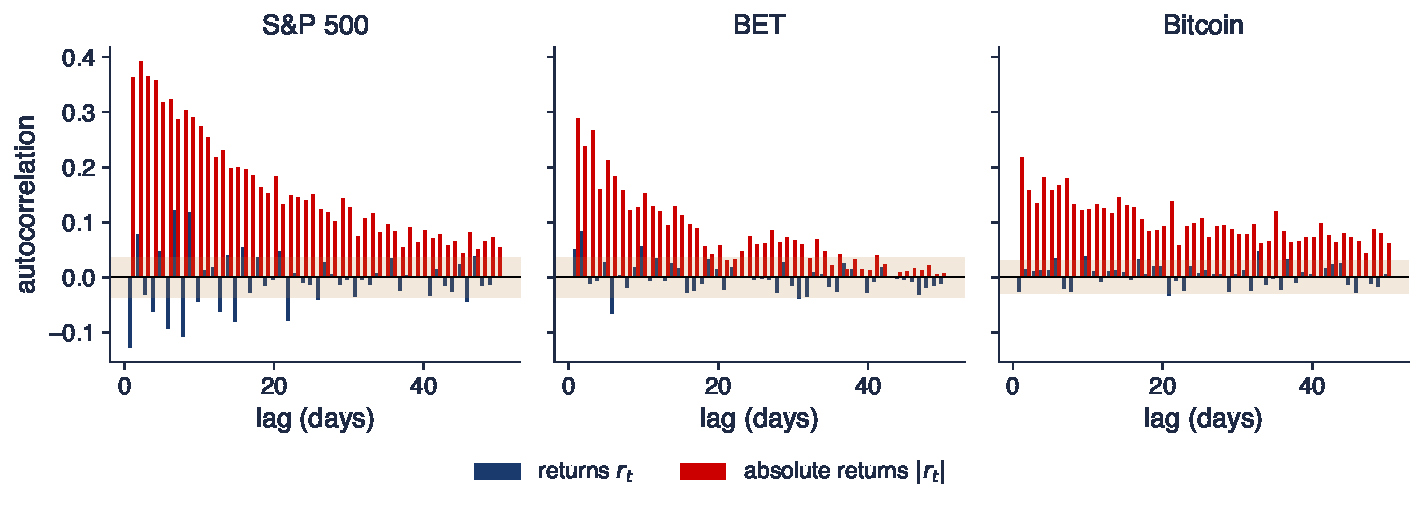
\includegraphics[width=0.97\textwidth,height=0.52\textheight,keepaspectratio]{sfm_ch16_stylised.pdf}
\end{center}
\vspace{-0.25cm}
\begin{itemize}
    \item Returns: autocorrelations small and mostly inside the band $\pm 1.96/\sqrt{T}$; absolute returns: positive for 50 days
    \item Uncorrelated is not independent: $\hat\rho_1(|r|) = 0.36$ (S\&P 500), $0.29$ (BET), $0.22$ (Bitcoin)
\end{itemize}
\sfmquantlet{Ch_16}{SFM_ch16_course_summary}
\end{frame}

\begin{frame}{Recap: The Course Map}
\itemsize{\small}
\begin{itemize}
    \item One chain in every chapter: data, distribution, dependence in time, risk, evaluation
    \item Three series carry the course: the S\&P 500 (a developed market), the BET (an emerging market), Bitcoin (a new asset class)
    \item All three: heavy tails, almost uncorrelated returns, strongly dependent volatility
\end{itemize}
\end{frame}


%=============================================================================
\section{Chapters 0--3: Data, Returns and Distributions}
%=============================================================================

\begin{frame}{\sfmchlinkt{https://danpele.github.io/SFM/EN/Courses/chapter0_introduction.pdf}{Chapter 0}: Introduction (1/2)}
\itemsize{\small}
\begin{itemize}
    \item \textbf{Key formulas}
    \begin{itemize}
        \item annualised volatility $\sigma_{\text{ann}} = \sqrt{A}\,\sigma$, $A$ = observations per year (252 for shares, 365 for crypto)
        \item drawdown $D_t = P_t/\max_{s \le t}P_s - 1$; maximum drawdown MDD $= \min_t D_t$
    \end{itemize}
    \item \textbf{Notation}
    \begin{itemize}
        \item $\sigma$: the standard deviation of daily returns; $A$: the number of observations per year
        \item $P_t$: the price on day $t$; $\max_{s \le t}P_s$: the highest price up to day $t$; $D_t \le 0$
    \end{itemize}
\end{itemize}
\end{frame}

\begin{frame}{\sfmchlinkt{https://danpele.github.io/SFM/EN/Courses/chapter0_introduction.pdf}{Chapter 0}: Introduction (2/2)}
\itemsize{\small}
\begin{itemize}
    \item \textbf{Empirical facts}
    \begin{itemize}
        \item since 2015: volatility 17.7\% a year for the S\&P 500, 66.7\% for Bitcoin
        \item BET: $-82.5\%$ from 24 July 2007 to 25 February 2009; back to the peak only on 16 March 2021
    \end{itemize}
    \item \textbf{Common mistakes}
    \begin{itemize}
        \item prices from several sources mixed, or unadjusted prices for shares with dividends and splits
        \item a referenced number or paper produced by AI and never checked
    \end{itemize}
\end{itemize}
\end{frame}

\begin{frame}{\sfmchlinkt{https://danpele.github.io/SFM/EN/Courses/chapter1_data_returns_indicators.pdf}{Chapter 1}: Data, Returns and Indicators (1/2)}
\itemsize{\small}
\begin{itemize}
    \item \textbf{Key formulas}
    \begin{itemize}
        \item $R_t = P_t/P_{t-1} - 1$, $r_t = \ln(1 + R_t)$; log returns add over time, simple returns add across assets
        \item CAGR $= (P_T/P_0)^{1/Y} - 1$; Sharpe $= (\mu - r_f)/\sigma$, SE $\approx \sqrt{(1 + \mathrm{SR}^2/2)/Y}$; volatility drag $\approx \sigma^2/2$
    \end{itemize}
    \item \textbf{Notation}
    \begin{itemize}
        \item $R_t$: the simple return, $r_t$: the log return of period $t$; $P_0$, $P_T$: the first and the last price; $Y$: the number of years
        \item $\mu$, $\sigma$: the annual mean and volatility; $r_f$: the risk-free rate; SR: the Sharpe ratio; SE: its standard error
    \end{itemize}
\end{itemize}
\end{frame}

\begin{frame}{\sfmchlinkt{https://danpele.github.io/SFM/EN/Courses/chapter1_data_returns_indicators.pdf}{Chapter 1}: Data, Returns and Indicators (2/2)}
\itemsize{\small}
\begin{itemize}
    \item \textbf{Empirical facts}
    \begin{itemize}
        \item BET since 2015: CAGR 14.1\%, volatility 15.4\%, Sharpe 0.93 with 95\% CI [0.36, 1.51]
        \item Bitcoin: arithmetic mean 69.5\% a year, CAGR only 60.6\%: the volatility drag
    \end{itemize}
    \item \textbf{Common mistakes}
    \begin{itemize}
        \item adding simple returns over time; averaging returns instead of computing the CAGR
        \item annualising with 252 for Bitcoin; reporting a Sharpe ratio without its standard error
    \end{itemize}
\end{itemize}
\end{frame}

\begin{frame}{\sfmchlinkt{https://danpele.github.io/SFM/EN/Courses/chapter2_classical_distributions_stylised_facts.pdf}{Chapter 2}: Classical Distributions and Stylised Facts (1/2)}
\itemsize{\small}
\begin{itemize}
    \item \textbf{Key formulas}
    \begin{itemize}
        \item $S = m_3/m_2^{3/2}$, $K = m_4/m_2^2 - 3$; $\text{JB} = \frac{n}{6}(S^2 + K^2/4) \sim \chi^2(2)$ \refJB
        \item Student-$t(\nu)$: excess kurtosis $6/(\nu - 4)$ for $\nu > 4$; Ljung--Box $Q(m) = n(n+2)\sum_h \hat\rho(h)^2/(n - h)$
    \end{itemize}
    \item \textbf{Notation}
    \begin{itemize}
        \item $m_k = \frac1n\sum_t (r_t - \bar r)^k$: the $k$-th central moment; $S$: skewness; $K$: excess kurtosis (0 for the Normal distribution)
        \item JB: Jarque--Bera, $\chi^2(2)$ under normality; $\nu$: degrees of freedom; $\hat\rho(h)$: the autocorrelation at lag $h$; $m$: the number of lags
    \end{itemize}
\end{itemize}
\end{frame}

\begin{frame}{\sfmchlinkt{https://danpele.github.io/SFM/EN/Courses/chapter2_classical_distributions_stylised_facts.pdf}{Chapter 2}: Classical Distributions and Stylised Facts (2/2)}
\itemsize{\small}
\begin{itemize}
    \item \textbf{Empirical facts}
    \begin{itemize}
        \item BET since 2010: $S = -0.98$, $K = 17.9$, JB $=$ 56\,762; fitted Student-$t$: $\hat\nu = 2.96$
        \item $\hat\rho_1(r) = 0.03$ but $\hat\rho_1(|r|) = 0.34$: the six stylised facts of \refCont
    \end{itemize}
    \item \textbf{Common mistakes}
    \begin{itemize}
        \item reading the kurtosis $K + 3$ as the excess kurtosis (the Normal distribution has kurtosis 3, excess 0)
        \item concluding independence from a non-significant ACF of $r_t$
    \end{itemize}
\end{itemize}
\end{frame}

\begin{frame}{\sfmchlinkt{https://danpele.github.io/SFM/EN/Courses/chapter3_alpha_stable_distributions.pdf}{Chapter 3}: $\alpha$-Stable Distributions (1/2)}
\itemsize{\small}
\begin{itemize}
    \item \textbf{Key formulas}
    \begin{itemize}
        \item $X_1 + \dots + X_n \overset{d}{=} n^{1/\alpha}X + d_n$; tails $P(X > x) \sim c\,x^{-\alpha}$; $E|X|^p < \infty$ only for $p < \alpha$
        \item four parameters: $\alpha$ (tails), $\beta$ (skewness), $\gamma$ (scale), $\delta$ (location), in S0 or S1 \refNolan
    \end{itemize}
    \item \textbf{Notation}
    \begin{itemize}
        \item $X_1, \dots, X_n$: independent copies of $X$; $\overset{d}{=}$: same distribution; $d_n$: a shift; $\alpha \in (0, 2]$: the stability index
        \item $c$: a constant; $p$: the order of a moment; S0, S1: two parametrisations of the same family
    \end{itemize}
\end{itemize}
\end{frame}

\begin{frame}{\sfmchlinkt{https://danpele.github.io/SFM/EN/Courses/chapter3_alpha_stable_distributions.pdf}{Chapter 3}: $\alpha$-Stable Distributions (2/2)}
\itemsize{\small}
\begin{itemize}
    \item \textbf{Empirical facts}
    \begin{itemize}
        \item maximum likelihood since 2000: $\hat\alpha = 1.49$ (BET), $1.54$ (S\&P 500), $1.41$ (Bitcoin), as \refMandelbrot{} found for cotton
        \item but the sample variance settles down and $\hat\alpha$ of the BET stays near 1.50 on monthly data: heavy tails with finite variance
    \end{itemize}
    \item \textbf{Common mistakes}
    \begin{itemize}
        \item using the standard deviation as a scale when $\alpha < 2$ (the variance does not exist)
        \item comparing $\delta$ from two programs that use different parametrisations
    \end{itemize}
\end{itemize}
\end{frame}

\begin{frame}{Recap: \sfmchlinkt{https://danpele.github.io/SFM/EN/Courses/chapter0_introduction.pdf}{Chapters 0}--\sfmchlinkt{https://danpele.github.io/SFM/EN/Courses/chapter3_alpha_stable_distributions.pdf}{3}}
\itemsize{\small}
\begin{itemize}
    \item Clean data and log returns first; annualise with the actual frequency
    \item Returns are not Normal: negative skewness, large excess kurtosis, JB rejects everywhere
    \item Stable laws fit the body well, but the variance of returns is finite
\end{itemize}
\end{frame}


%=============================================================================
\section{Chapters 4--7: Probability, Tails, Model Choice, Efficiency}
%=============================================================================

\begin{frame}{\sfmchlinkt{https://danpele.github.io/SFM/EN/Courses/chapter4_probability.pdf}{Chapter 4}: Probability (1/2)}
\itemsize{\small}
\begin{itemize}
    \item \textbf{Key formulas}
    \begin{itemize}
        \item $\mathrm{Var}(aX + bY) = a^2\sigma_X^2 + b^2\sigma_Y^2 + 2ab\,\mathrm{Cov}(X, Y)$; Monte Carlo error $\sqrt{p(1 - p)/N}$
        \item GBM: $S_t = S_0\exp((\mu - \sigma^2/2)t + \sigma W_t)$, mean $S_0e^{\mu t}$, median $S_0e^{(\mu - \sigma^2/2)t}$
    \end{itemize}
    \item \textbf{Notation}
    \begin{itemize}
        \item $a$, $b$: weights; $\sigma_X$, $\sigma_Y$: standard deviations; $p$: the estimated probability; $N$: the number of Monte Carlo draws
        \item GBM (geometric Brownian motion): $S_t$: price at time $t$ (years); $\mu$: drift; $\sigma$: volatility; $W_t \sim N(0, t)$: a Brownian motion
    \end{itemize}
\end{itemize}
\end{frame}

\begin{frame}{\sfmchlinkt{https://danpele.github.io/SFM/EN/Courses/chapter4_probability.pdf}{Chapter 4}: Probability (2/2)}
\itemsize{\small}
\begin{itemize}
    \item \textbf{Empirical facts}
    \begin{itemize}
        \item S\&P 500 since 2000: a day below $-5\%$ has frequency 0.34\%; the Normal distribution gives 0.0017\%, 199 times less
        \item mean return 6.2\% a year with SE 3.7\%: about 86 years of data would be needed for $t = 3$
    \end{itemize}
    \item \textbf{Common mistakes}
    \begin{itemize}
        \item uncorrelated taken for independent; the mean of $S_t$ taken for its median
        \item a Monte Carlo estimate without its standard error
    \end{itemize}
\end{itemize}
\end{frame}

\begin{frame}{\sfmchlinkt{https://danpele.github.io/SFM/EN/Courses/chapter5_heavy_tails_evt.pdf}{Chapter 5}: Heavy Tails and Extreme Value Theory (1/2)}
\itemsize{\small}
\begin{itemize}
    \item \textbf{Key formulas}
    \begin{itemize}
        \item Hill: $\hat\alpha_k = [\frac1k\sum_{i=1}^k \ln(L_{(i)}/L_{(k+1)})]^{-1}$, SE $\approx \hat\alpha/\sqrt{k}$ \refHill; $\xi = 1/\alpha$
        \item GPD above $u$: VaR $= u + \frac{\beta}{\xi}[(n\alpha/N_u)^{-\xi} - 1]$; GEV for block maxima
    \end{itemize}
    \item \textbf{Notation}
    \begin{itemize}
        \item $L_{(i)}$: the $i$-th largest loss; $k$: the number of tail observations; $\xi = 1/\alpha$: the shape (tail) parameter
        \item GPD: $u$: the threshold; $\beta$: the scale; $N_u$: the losses above $u$ out of $n$; in the VaR formula $\alpha$ is the level (1\%), not the tail index
    \end{itemize}
\end{itemize}
\end{frame}

\begin{frame}{\sfmchlinkt{https://danpele.github.io/SFM/EN/Courses/chapter5_heavy_tails_evt.pdf}{Chapter 5}: Heavy Tails and Extreme Value Theory (2/2)}
\itemsize{\small}
\begin{itemize}
    \item \textbf{Empirical facts}
    \begin{itemize}
        \item tail index of the losses: BET 2.57 (95\% CI [2.20, 2.95], since 1997), S\&P 500 2.97, Bitcoin 2.71
        \item BET, VaR 0.1\%: EVT 9.6\%, Normal only 4.5\%
    \end{itemize}
    \item \textbf{Common mistakes}
    \begin{itemize}
        \item choosing $k$ without looking at the Hill plot; reporting $\hat\alpha$ without an interval
        \item applying the Hill estimator to returns instead of losses $L = -r$
    \end{itemize}
\end{itemize}
\end{frame}

\begin{frame}{\sfmchlinkt{https://danpele.github.io/SFM/EN/Courses/chapter6_model_selection_risk_management.pdf}{Chapter 6}: Model Selection and Risk Management (1/2)}
\itemsize{\small}
\begin{itemize}
    \item \textbf{Key formulas}
    \begin{itemize}
        \item $LR = 2(\ell_1 - \ell_0) \approx \chi^2(k_1 - k_0)$ for nested models; AIC $= -2\ell + 2k$, BIC $= -2\ell + k\ln n$
        \item KS: $D_n = \sup_x|F_n(x) - F(x)|$; Anderson--Darling weights the tails
    \end{itemize}
    \item \textbf{Notation}
    \begin{itemize}
        \item $\ell_0$, $\ell_1$: the maximised log-likelihoods of the smaller and of the larger model; $k_0$, $k_1$, $k$: numbers of parameters; $n$: sample size
        \item $F_n$: the empirical distribution function; $F$: the model; $D_n$: their largest vertical distance; smaller AIC or BIC is better
    \end{itemize}
\end{itemize}
\end{frame}

\begin{frame}{\sfmchlinkt{https://danpele.github.io/SFM/EN/Courses/chapter6_model_selection_risk_management.pdf}{Chapter 6}: Model Selection and Risk Management (2/2)}
\itemsize{\small}
\begin{itemize}
    \item \textbf{Empirical facts}
    \begin{itemize}
        \item BET since 2000, Anderson--Darling: Normal 161, Student-$t$ 0.54, NIG 0.40
        \item VaR 1\% of the BET: Normal 3.19\%, heavy-tailed models 3.74--4.94\%
    \end{itemize}
    \item \textbf{Common mistakes}
    \begin{itemize}
        \item the LR test at the boundary (e.g.\ $\nu = \infty$) without the corrected critical value
        \item rejecting every model with a large $n$ and stopping there, instead of ranking the models
    \end{itemize}
\end{itemize}
\end{frame}

\begin{frame}{\sfmchlinkt{https://danpele.github.io/SFM/EN/Courses/chapter7_efficient_markets_random_walk_vr.pdf}{Chapter 7}: Efficient Markets, Random Walk and VR Tests (1/2)}
\itemsize{\small}
\begin{itemize}
    \item \textbf{Key formulas}
    \begin{itemize}
        \item weak-form efficiency: past prices do not predict excess returns \refFama; null: martingale differences
        \item $\mathrm{VR}(q) = 1 + 2\sum_{k=1}^{q-1}(1 - k/q)\rho(k)$; robust $Z^*(q) = (\widehat{\mathrm{VR}} - 1)/\sqrt{\hat\theta/T}$ \refLM
    \end{itemize}
    \item \textbf{Notation}
    \begin{itemize}
        \item $\rho(k)$: the autocorrelation at lag $k$; $q$: the horizon of the variance ratio; VR $= 1$ under a random walk
        \item $T$: the number of returns; $\hat\theta$: a variance estimate robust to volatility clustering; $Z^* \approx N(0, 1)$ under the null
    \end{itemize}
\end{itemize}
\end{frame}

\begin{frame}{\sfmchlinkt{https://danpele.github.io/SFM/EN/Courses/chapter7_efficient_markets_random_walk_vr.pdf}{Chapter 7}: Efficient Markets, Random Walk and VR Tests (2/2)}
\itemsize{\small}
\begin{itemize}
    \item \textbf{Empirical facts}
    \begin{itemize}
        \item BET since 1997: VR(5) $= 1.28$, $Z^* = 5.25$ (momentum)
        \item S\&P 500 since 1990: VR(5) $= 0.86$, $Z^* = -2.76$ (mean reversion); Bitcoin: $Z^* = -0.19$
    \end{itemize}
    \item \textbf{Common mistakes}
    \begin{itemize}
        \item the i.i.d. statistic $Z(q)$ on returns with volatility clustering (it rejects too often)
        \item a unit root in prices read as proof of efficiency; predictability read as profit
    \end{itemize}
\end{itemize}
\end{frame}

\begin{frame}{Recap: \sfmchlinkt{https://danpele.github.io/SFM/EN/Courses/chapter4_probability.pdf}{Chapters 4}--\sfmchlinkt{https://danpele.github.io/SFM/EN/Courses/chapter7_efficient_markets_random_walk_vr.pdf}{7}}
\itemsize{\small}
\begin{itemize}
    \item Probability gives the tools: covariance, conditional variance, Monte Carlo with its error
    \item Tails are power laws with $\alpha$ between 2 and 4; EVT gives VaR far in the tail
    \item Choose the model for its purpose and check it out of sample; test efficiency with robust statistics
\end{itemize}
\end{frame}


%=============================================================================
\section{Chapters 8--11: Volatility, Risk and Memory}
%=============================================================================

\begin{frame}{\sfmchlinkt{https://danpele.github.io/SFM/EN/Courses/chapter8_volatility_estimators.pdf}{Chapter 8}: Volatility Estimators (1/2)}
\itemsize{\small}
\begin{itemize}
    \item \textbf{Key formulas}
    \begin{itemize}
        \item EWMA: $\sigma_t^2 = \lambda\sigma_{t-1}^2 + (1 - \lambda)r_{t-1}^2$, half-life $\ln 0.5/\ln\lambda$ \refRM
        \item Parkinson: $(\ln H_t - \ln L_t)^2/(4\ln 2)$; ARCH-LM $= nR^2 \sim \chi^2(q)$
    \end{itemize}
    \item \textbf{Notation}
    \begin{itemize}
        \item $\lambda \in (0, 1)$: the decay factor; $r_{t-1}$: yesterday's return; $H_t$, $L_t$: the high and the low of day $t$
        \item ARCH-LM: $R^2$ of the regression of $r_t^2$ on its $q$ lags, times $n$; a large value: volatility clustering
    \end{itemize}
\end{itemize}
\end{frame}

\begin{frame}{\sfmchlinkt{https://danpele.github.io/SFM/EN/Courses/chapter8_volatility_estimators.pdf}{Chapter 8}: Volatility Estimators (2/2)}
\itemsize{\small}
\begin{itemize}
    \item \textbf{Empirical facts}
    \begin{itemize}
        \item S\&P 500: Ljung--Box $Q(10)$ is 91 on $r_t$ and 8015 on $r_t^2$ (critical value 18.31)
        \item EWMA with $\lambda = 0.94$: half-life of 11.2 days; no ghost effect
    \end{itemize}
    \item \textbf{Common mistakes}
    \begin{itemize}
        \item a rolling window of fixed length: one extreme day enters and leaves abruptly (ghost effect)
        \item range estimators on prices with overnight gaps, without the Yang--Zhang correction
    \end{itemize}
\end{itemize}
\end{frame}

\begin{frame}{\sfmchlinkt{https://danpele.github.io/SFM/EN/Courses/chapter9_arch_garch_models.pdf}{Chapter 9}: ARCH and GARCH Models (1/2)}
\itemsize{\small}
\begin{itemize}
    \item \textbf{Key formulas}
    \begin{itemize}
        \item GARCH(1,1): $\sigma_t^2 = \omega + \alpha\varepsilon_{t-1}^2 + \beta\sigma_{t-1}^2$, $\bar\sigma^2 = \omega/(1 - \alpha - \beta)$ \refEngle, \refBoll
        \item forecast $E_t\sigma_{t+h}^2 = \bar\sigma^2 + (\alpha + \beta)^{h-1}(\sigma_{t+1}^2 - \bar\sigma^2)$; half-life $\ln 0.5/\ln(\alpha + \beta)$
    \end{itemize}
    \item \textbf{Notation}
    \begin{itemize}
        \item $\omega$: the constant; $\alpha$: the reaction to yesterday's shock $\varepsilon_{t-1}$; $\beta$: the memory; $\bar\sigma^2$: the long-run variance
        \item $E_t$: the forecast made at day $t$; $h$: the horizon in days; $\alpha + \beta$: the speed at which the forecast returns to $\bar\sigma^2$
    \end{itemize}
\end{itemize}
\end{frame}

\begin{frame}{\sfmchlinkt{https://danpele.github.io/SFM/EN/Courses/chapter9_arch_garch_models.pdf}{Chapter 9}: ARCH and GARCH Models (2/2)}
\itemsize{\small}
\begin{itemize}
    \item \textbf{Empirical facts}
    \begin{itemize}
        \item GARCH(1,1)-$t$ since 2000: $\alpha + \beta = 0.995$ (S\&P 500, half-life 131 days), $0.991$ (BET, 74 days)
        \item Bitcoin: $\alpha + \beta = 1.000$, an IGARCH; equity indices need asymmetry (GJR, EGARCH)
    \end{itemize}
    \item \textbf{Common mistakes}
    \begin{itemize}
        \item Normal innovations for returns with heavy tails; non-robust standard errors
        \item a long-run variance $\omega/(1 - \alpha - \beta)$ reported when $\alpha + \beta \ge 1$
    \end{itemize}
\end{itemize}
\end{frame}

\begin{frame}{\sfmchlinkt{https://danpele.github.io/SFM/EN/Courses/chapter10_var_es_backtesting.pdf}{Chapter 10}: VaR, ES and Backtesting (1/2)}
\itemsize{\small}
\begin{itemize}
    \item \textbf{Key formulas}
    \begin{itemize}
        \item $\mathrm{VaR}_\alpha = -q_\alpha(X)$, $\mathrm{ES}_\alpha = -\frac1\alpha\int_0^\alpha q_u\,du$; Normal: $-(\mu + \sigma z_\alpha)$, $-\mu + \sigma\varphi(z_\alpha)/\alpha$
        \item Kupiec: $LR_{uc} = -2\ln[(1-\alpha)^{n-x}\alpha^x/((1-\hat\pi)^{n-x}\hat\pi^x)] \sim \chi^2(1)$ \refKupiec; ES is coherent \refArtzner
    \end{itemize}
    \item \textbf{Notation}
    \begin{itemize}
        \item $q_\alpha$: the $\alpha$-quantile of the return $X$; $z_\alpha$: the standard Normal quantile; $\varphi$: the standard Normal density
        \item $x$: the exceptions in $n$ days; $\hat\pi = x/n$: the observed rate; $LR_{uc}$ compares it with the target $\alpha$
    \end{itemize}
\end{itemize}
\end{frame}

\begin{frame}{\sfmchlinkt{https://danpele.github.io/SFM/EN/Courses/chapter10_var_es_backtesting.pdf}{Chapter 10}: VaR, ES and Backtesting (2/2)}
\itemsize{\small}
\begin{itemize}
    \item \textbf{Empirical facts}
    \begin{itemize}
        \item S\&P 500, VaR 1\%: historical 3.46\%, Normal 2.80\%, i.e.\ 19\% too low
        \item exception rates since 2005: Normal 2.71\%, HS 1.41\%, GARCH-$t$ 1.74\%, FHS 1.58\% (target 1\%)
    \end{itemize}
    \item \textbf{Common mistakes}
    \begin{itemize}
        \item a negative VaR or ``VaR 99\%'': the course writes VaR 1\%, a positive loss
        \item $\sqrt{10}$ scaling as if returns were i.i.d.\ Normal; checking only the number of exceptions, not their clustering
    \end{itemize}
\end{itemize}
\end{frame}

\begin{frame}{VaR 1\% Forecasts of the BET: Historical Simulation and EWMA-Normal}
\itemsize{\footnotesize}
\begin{center}
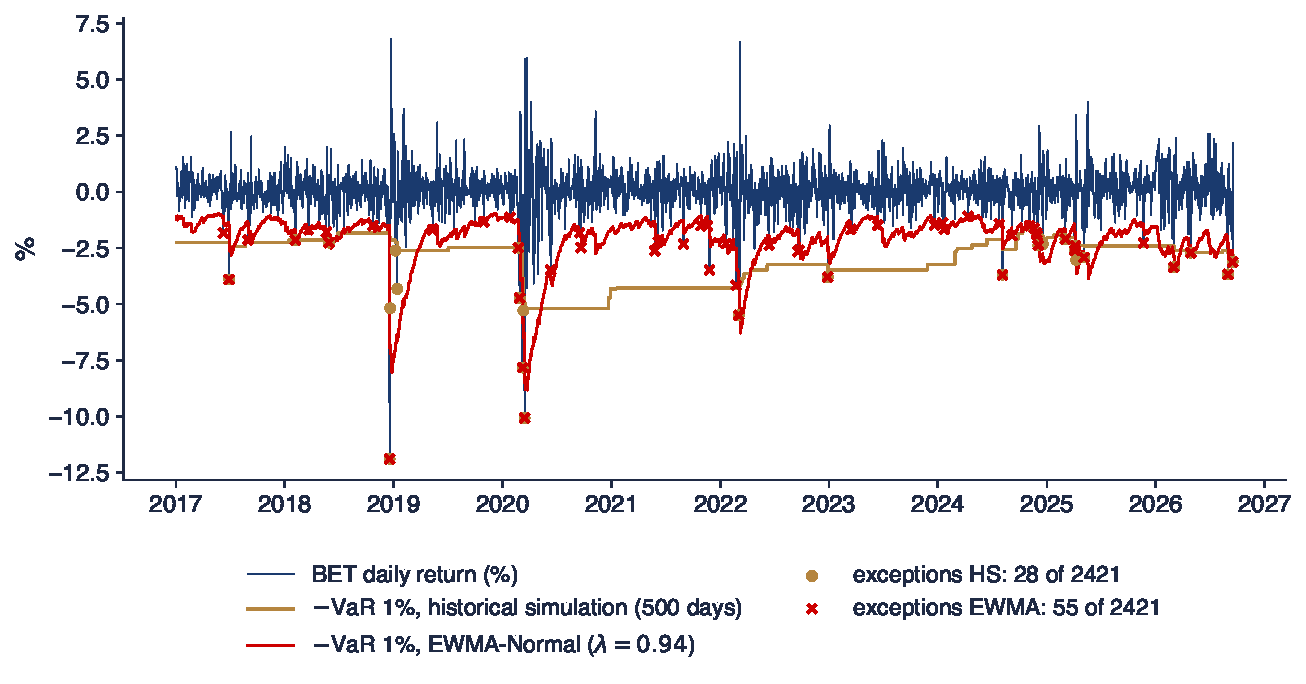
\includegraphics[width=0.97\textwidth,height=0.56\textheight,keepaspectratio]{sfm_ch16_backtest.pdf}
\end{center}
\vspace{-0.25cm}
\begin{itemize}
    \item Since 3 January 2017, 2\,421 days, 24.2 expected exceptions: HS 28 (1.16\%, Kupiec $p = 0.450$), EWMA-Normal 55 (2.27\%, $p$ $<$\,0.001)
    \item EWMA follows the storms, but the Normal quantile is too small; HS has the right rate, but its exceptions come in clusters (at most 10 in 250 days)
\end{itemize}
\sfmquantlet{Ch_16}{SFM_ch16_course_summary}
\end{frame}

\begin{frame}{\sfmchlinkt{https://danpele.github.io/SFM/EN/Courses/chapter11_fractal_markets_long_memory.pdf}{Chapter 11}: Fractal Markets Hypothesis and Long Memory (1/2)}
\itemsize{\small}
\begin{itemize}
    \item \textbf{Key formulas}
    \begin{itemize}
        \item $(R/S)_n \propto n^H$ \refHurst; $H = 0.5$: no memory, $H > 0.5$: persistence; $d = H - 0.5$
        \item risk scaling: $\mathrm{sd}(r^{(h)}) = h^H\mathrm{sd}(r)$; fractal markets need many investment horizons \refPeters
    \end{itemize}
    \item \textbf{Notation}
    \begin{itemize}
        \item $(R/S)_n$: the rescaled range (range of the cumulated deviations divided by the standard deviation) on blocks of $n$ days
        \item $H$: the Hurst exponent; $d$: the fractional parameter; $r^{(h)}$: the $h$-day return; sd: the standard deviation
    \end{itemize}
\end{itemize}
\end{frame}

\begin{frame}{\sfmchlinkt{https://danpele.github.io/SFM/EN/Courses/chapter11_fractal_markets_long_memory.pdf}{Chapter 11}: Fractal Markets Hypothesis and Long Memory (2/2)}
\itemsize{\small}
\begin{itemize}
    \item \textbf{Empirical facts}
    \begin{itemize}
        \item BET: $H$ (R/S) $= 0.58$ for $r_t$, at the edge of the Monte Carlo band, and the Lo test rejects: weak persistence; $0.79$ for $|r_t|$
        \item S\&P 500: $0.53$ for returns, $0.86$ for absolute returns: long memory is in the volatility
    \end{itemize}
    \item \textbf{Common mistakes}
    \begin{itemize}
        \item comparing $\hat H$ with 0.5 instead of a Monte Carlo band for the same $N$ (R/S is biased upwards)
        \item structural breaks or GARCH taken for long memory
    \end{itemize}
\end{itemize}
\end{frame}

\begin{frame}{Recap: \sfmchlinkt{https://danpele.github.io/SFM/EN/Courses/chapter8_volatility_estimators.pdf}{Chapters 8}--\sfmchlinkt{https://danpele.github.io/SFM/EN/Courses/chapter11_fractal_markets_long_memory.pdf}{11}}
\itemsize{\small}
\begin{itemize}
    \item Volatility is latent, persistent and predictable: EWMA and GARCH forecast it
    \item A risk number needs both a volatility forecast and a heavy-tailed quantile, and then a backtest
    \item Long memory: weak in returns, strong in volatility
\end{itemize}
\end{frame}


%=============================================================================
\section{Chapters 12--15: Applications}
%=============================================================================

\begin{frame}{\sfmchlinkt{https://danpele.github.io/SFM/EN/Courses/chapter12_scoring_models.pdf}{Chapter 12}: Scoring Models (1/2)}
\itemsize{\small}
\begin{itemize}
    \item \textbf{Key formulas}
    \begin{itemize}
        \item EL $=$ PD $\times$ LGD $\times$ EAD; logit $\ln\frac{p}{1-p} = \beta_0 + x^\top\beta$, $e^{\beta_j}$ = odds ratio
        \item AUC $= P(s_{\text{bad}} > s_{\text{good}})$, Gini $= 2\,\mathrm{AUC} - 1$; Altman $Z$ and Merton distance to default \refAltman
    \end{itemize}
    \item \textbf{Notation}
    \begin{itemize}
        \item EL: expected loss; PD: probability of default; LGD: loss given default; EAD: exposure at default
        \item $p$: the probability of default given $x$; $\beta_j$: a coefficient; $s$: the score of a bad or a good borrower; AUC $= 0.5$: no discrimination, 1: perfect
    \end{itemize}
\end{itemize}
\end{frame}

\begin{frame}{\sfmchlinkt{https://danpele.github.io/SFM/EN/Courses/chapter12_scoring_models.pdf}{Chapter 12}: Scoring Models (2/2)}
\itemsize{\small}
\begin{itemize}
    \item \textbf{Empirical facts}
    \begin{itemize}
        \item German credit data (1000 loans), test sample of 300: AUC $= 0.801$, 95\% CI [0.75, 0.85], Gini 0.60
        \item discrimination is not calibration: check both, out of sample
    \end{itemize}
    \item \textbf{Common mistakes}
    \begin{itemize}
        \item accuracy on imbalanced classes (always ``good'' is already right in most cases)
        \item choosing the cut-off without the costs of the two errors
    \end{itemize}
\end{itemize}
\end{frame}

\begin{frame}{\sfmchlinkt{https://danpele.github.io/SFM/EN/Courses/chapter13_machine_learning.pdf}{Chapter 13}: Machine Learning (1/2)}
\itemsize{\small}
\begin{itemize}
    \item \textbf{Key formulas}
    \begin{itemize}
        \item bias--variance: $E(y_0 - \hat f)^2 = \text{bias}^2 + \mathrm{Var}(\hat f) + \sigma^2$; ridge, lasso, trees, boosting
        \item out of sample: $R^2_{OOS} = 1 - \sum(y - \hat y)^2/\sum(y - \tilde y)^2$ against a simple benchmark $\tilde y$ \refGKX
    \end{itemize}
    \item \textbf{Notation}
    \begin{itemize}
        \item $y_0$: a new observation; $\hat f$: the fitted model; $\sigma^2$: the noise variance; $\hat y$: the forecast
        \item $\tilde y$: the benchmark forecast; sums over the test sample; $R^2_{OOS} < 0$: worse than the benchmark
    \end{itemize}
\end{itemize}
\end{frame}

\begin{frame}{\sfmchlinkt{https://danpele.github.io/SFM/EN/Courses/chapter13_machine_learning.pdf}{Chapter 13}: Machine Learning (2/2)}
\itemsize{\small}
\begin{itemize}
    \item \textbf{Empirical facts}
    \begin{itemize}
        \item sign of S\&P 500 returns since 2008: ``always up'' 54.4\%, logit 53.8\%, boosting 52.1\%
        \item realised volatility: HAR $R^2_{OOS} = 0.61$ against the mean; lasso lowers the squared error of HAR by only 7.1\%
    \end{itemize}
    \item \textbf{Common mistakes}
    \begin{itemize}
        \item random cross-validation on time series (look-ahead bias and leakage)
        \item reporting the best of many trials without deflating the Sharpe ratio
    \end{itemize}
\end{itemize}
\end{frame}

\begin{frame}{\sfmchlinkt{https://danpele.github.io/SFM/EN/Courses/chapter14_crypto_assets.pdf}{Chapter 14}: Crypto Assets (1/2)}
\itemsize{\small}
\begin{itemize}
    \item \textbf{Key formulas}
    \begin{itemize}
        \item annualise with 365 days: $\sigma_{\text{ann}} = \sqrt{365}\,\sigma$; supply of Bitcoin capped at 21 million \refNakamoto
        \item peg deviation of a stablecoin $d_t = 10\,000\,(P_t - 1)$ basis points
    \end{itemize}
    \item \textbf{Notation}
    \begin{itemize}
        \item $\sigma$: the standard deviation of daily returns; crypto trades 365 days a year
        \item $P_t$: the price of the stablecoin in USD; 1 basis point $= 0.01\%$; $d_t < 0$: below the peg
    \end{itemize}
\end{itemize}
\end{frame}

\begin{frame}{\sfmchlinkt{https://danpele.github.io/SFM/EN/Courses/chapter14_crypto_assets.pdf}{Chapter 14}: Crypto Assets (2/2)}
\itemsize{\small}
\begin{itemize}
    \item \textbf{Empirical facts}
    \begin{itemize}
        \item Bitcoin: volatility 66.6\% a year with 365 days (55.3\% if one wrongly uses 252), maximum drawdown $-83.4\%$
        \item correlation with the S\&P 500: 0.02 before 2020, 0.39 after: not a safe haven
    \end{itemize}
    \item \textbf{Common mistakes}
    \begin{itemize}
        \item removing weekends from crypto data, or joining crypto and equity returns on different calendars
        \item a Normal VaR for a series with $\alpha + \beta = 1$ and tail index below 3
    \end{itemize}
\end{itemize}
\end{frame}

\begin{frame}{\sfmchlinkt{https://danpele.github.io/SFM/EN/Courses/chapter15_systemic_risk.pdf}{Chapter 15}: Systemic Risk (1/2)}
\itemsize{\small}
\begin{itemize}
    \item \textbf{Key formulas}
    \begin{itemize}
        \item CoVaR: the VaR of the system given an institution at its VaR; $\Delta\mathrm{CoVaR} = b\,(q_{50} - q_\alpha)$ from a quantile regression \refAB
        \item MES, SRISK, Granger networks and the Diebold--Yilmaz connectedness table \refDY
    \end{itemize}
    \item \textbf{Notation}
    \begin{itemize}
        \item $b$: the slope of the quantile regression of the system on the bank; $q_\alpha$, $q_{50}$: the $\alpha$-quantile and the median of the bank's return
        \item MES: the bank's mean loss on the market's worst days; SRISK: the capital missing in a crisis
    \end{itemize}
\end{itemize}
\end{frame}

\begin{frame}{\sfmchlinkt{https://danpele.github.io/SFM/EN/Courses/chapter15_systemic_risk.pdf}{Chapter 15}: Systemic Risk (2/2)}
\itemsize{\small}
\begin{itemize}
    \item \textbf{Empirical facts}
    \begin{itemize}
        \item Banca Transilvania and the BET: VaR 1\% 5.23\%, $\Delta$CoVaR 1\% 3.31 pp (95\% CI [2.35, 4.78])
        \item 11 US and European banks: total connectedness of about 78\%
    \end{itemize}
    \item \textbf{Common mistakes}
    \begin{itemize}
        \item ranking banks by their own VaR: a large VaR need not mean a large contribution to the system
        \item correlations compared across calm and crisis periods without the Forbes--Rigobon adjustment
    \end{itemize}
\end{itemize}
\end{frame}

\begin{frame}{Recap: \sfmchlinkt{https://danpele.github.io/SFM/EN/Courses/chapter12_scoring_models.pdf}{Chapters 12}--\sfmchlinkt{https://danpele.github.io/SFM/EN/Courses/chapter15_systemic_risk.pdf}{15}}
\itemsize{\small}
\begin{itemize}
    \item Scoring: discrimination (AUC, Gini) and calibration, out of sample, with costs
    \item Machine learning: judged against a simple benchmark, with walk-forward validation
    \item Crypto and systemic risk: the same tools, with the right calendar and conditional tail measures
\end{itemize}
\end{frame}


%=============================================================================
\section{The Toolbox}
%=============================================================================

\begin{frame}{Toolbox (1/2): Returns, Distributions and Tails}
\itemsize{\small}
\begin{center}
\footnotesize
\begin{tabular}{>{\raggedright\arraybackslash}p{3.6cm}>{\raggedright\arraybackslash}p{3.4cm}>{\raggedright\arraybackslash}p{3.4cm}c}
\toprule
\textbf{Question} & \textbf{Tool} & \textbf{Decision} & \textbf{Ch.} \\
\midrule
How good was the investment? & CAGR, Sharpe, Sortino, MDD & compare with SE and a benchmark & 1 \\
Are returns Normal? & JB, QQ plot & reject if JB $> 5.99$ & 2 \\
How heavy are the tails? & Hill plot, GPD, stable $\alpha$ & moments exist for $p < \alpha$ & 3, 5 \\
Which distribution fits? & LR, AIC, BIC, KS, AD & smallest AIC; AD for the tails & 6 \\
How rare is a loss of $x$? & empirical CDF, EVT, Monte Carlo & report the SE of the estimate & 4, 5 \\
Is the variance finite? & running variance, aggregation of $\hat\alpha$ & stable sample variance: finite & 3 \\
\bottomrule
\end{tabular}
\end{center}
\end{frame}

\begin{frame}{Toolbox (2/2): Dependence in Time, Volatility and Risk}
\itemsize{\small}
\begin{center}
\footnotesize
\begin{tabular}{>{\raggedright\arraybackslash}p{3.6cm}>{\raggedright\arraybackslash}p{3.4cm}>{\raggedright\arraybackslash}p{3.4cm}c}
\toprule
\textbf{Question} & \textbf{Tool} & \textbf{Decision} & \textbf{Ch.} \\
\midrule
Are returns predictable? & ACF, Ljung--Box, robust VR $Z^*(q)$ & reject if $|Z^*| > 1.96$ & 7 \\
Is there volatility clustering? & Ljung--Box on $r_t^2$, ARCH-LM & reject: model the variance & 8 \\
How volatile tomorrow? & EWMA, GARCH(1,1)-$t$, GJR & QLIKE against a benchmark & 8, 9 \\
How much can we lose? & VaR 1\%, ES 2.5\%: HS, $t$, EVT, FHS & Kupiec, Christoffersen, traffic light & 10 \\
Is there long memory? & R/S, DFA, GPH, Lo test & compare with a Monte Carlo band & 11 \\
Who will default? & logit, LDA, AUC, Gini & out of sample, with costs & 12 \\
Which bank matters for the system? & CoVaR, MES, SRISK & bootstrap CI of $\Delta$CoVaR & 15 \\
\bottomrule
\end{tabular}
\end{center}
\end{frame}

\begin{frame}{Conventions Used Throughout the Course}
\itemsize{\small}
\begin{itemize}
    \item \textbf{Returns}: daily log returns in \%, $r_t = 100\,(\ln P_t - \ln P_{t-1})$
    \begin{itemize}
        \item portfolios: simple returns, prices joined on common days first
    \end{itemize}
    \item \textbf{Annualisation}: mean $\times A$, volatility $\times\sqrt{A}$, with the actual $A$
    \begin{itemize}
        \item $A$: the number of observations per year: about 252 for shares and indices, 365 for crypto
    \end{itemize}
    \item \textbf{Risk}: the level is the tail probability: VaR 1\%, ES 2.5\%
    \begin{itemize}
        \item $\mathrm{VaR}_\alpha = -q_\alpha > 0$, a loss; historical simulation with $k = \lceil n\alpha \rceil$
    \end{itemize}
    \item \textbf{Tests}: state $H_0$, the statistic, its distribution, the critical value and the decision at 5\%
    \begin{itemize}
        \item then one sentence on what the decision means for the data
    \end{itemize}
\end{itemize}
\end{frame}

\begin{frame}{Six Pitfalls Across the Course}
\itemsize{\small}
\begin{itemize}
    \item \textbf{Data}: aligning returns instead of prices; unadjusted prices; weekends dropped from crypto
    \item \textbf{Distribution}: the Normal distribution for tail quantiles; excess kurtosis confused with kurtosis
    \item \textbf{Inference}: i.i.d. standard errors with volatility clustering; a statistic without its SE
    \item \textbf{Time}: look-ahead bias, parameters estimated on the whole sample and used in the past
    \item \textbf{Risk}: the sign and the level of VaR; ES compared with VaR at different levels
    \item \textbf{Interpretation}: significance taken for economic importance, predictability for profit
\end{itemize}
\end{frame}


%=============================================================================
\section{The Exam}
%=============================================================================

\begin{frame}{The Written Exam: Format}
\itemsize{\small}
\begin{columns}[T]
\begin{column}{0.58\textwidth}
\begin{itemize}
    \item \textbf{70\% of the final grade}; written, 2 hours; a calculator is allowed
    \begin{itemize}
        \item all subjects are compulsory; 9 points plus 1 point ex officio
    \end{itemize}
    \item \textbf{Useful values are given} on the paper
    \begin{itemize}
        \item quantiles of the Normal and Student-$t$ distributions, critical values of $\chi^2$, logarithms and square roots
    \end{itemize}
    \item \textbf{Each subject}: a short context, numbers or a table or a chart, one or two questions
    \begin{itemize}
        \item a computation, followed by an interpretation in three to five sentences
    \end{itemize}
\end{itemize}
\end{column}
\begin{column}{0.38\textwidth}
\centering
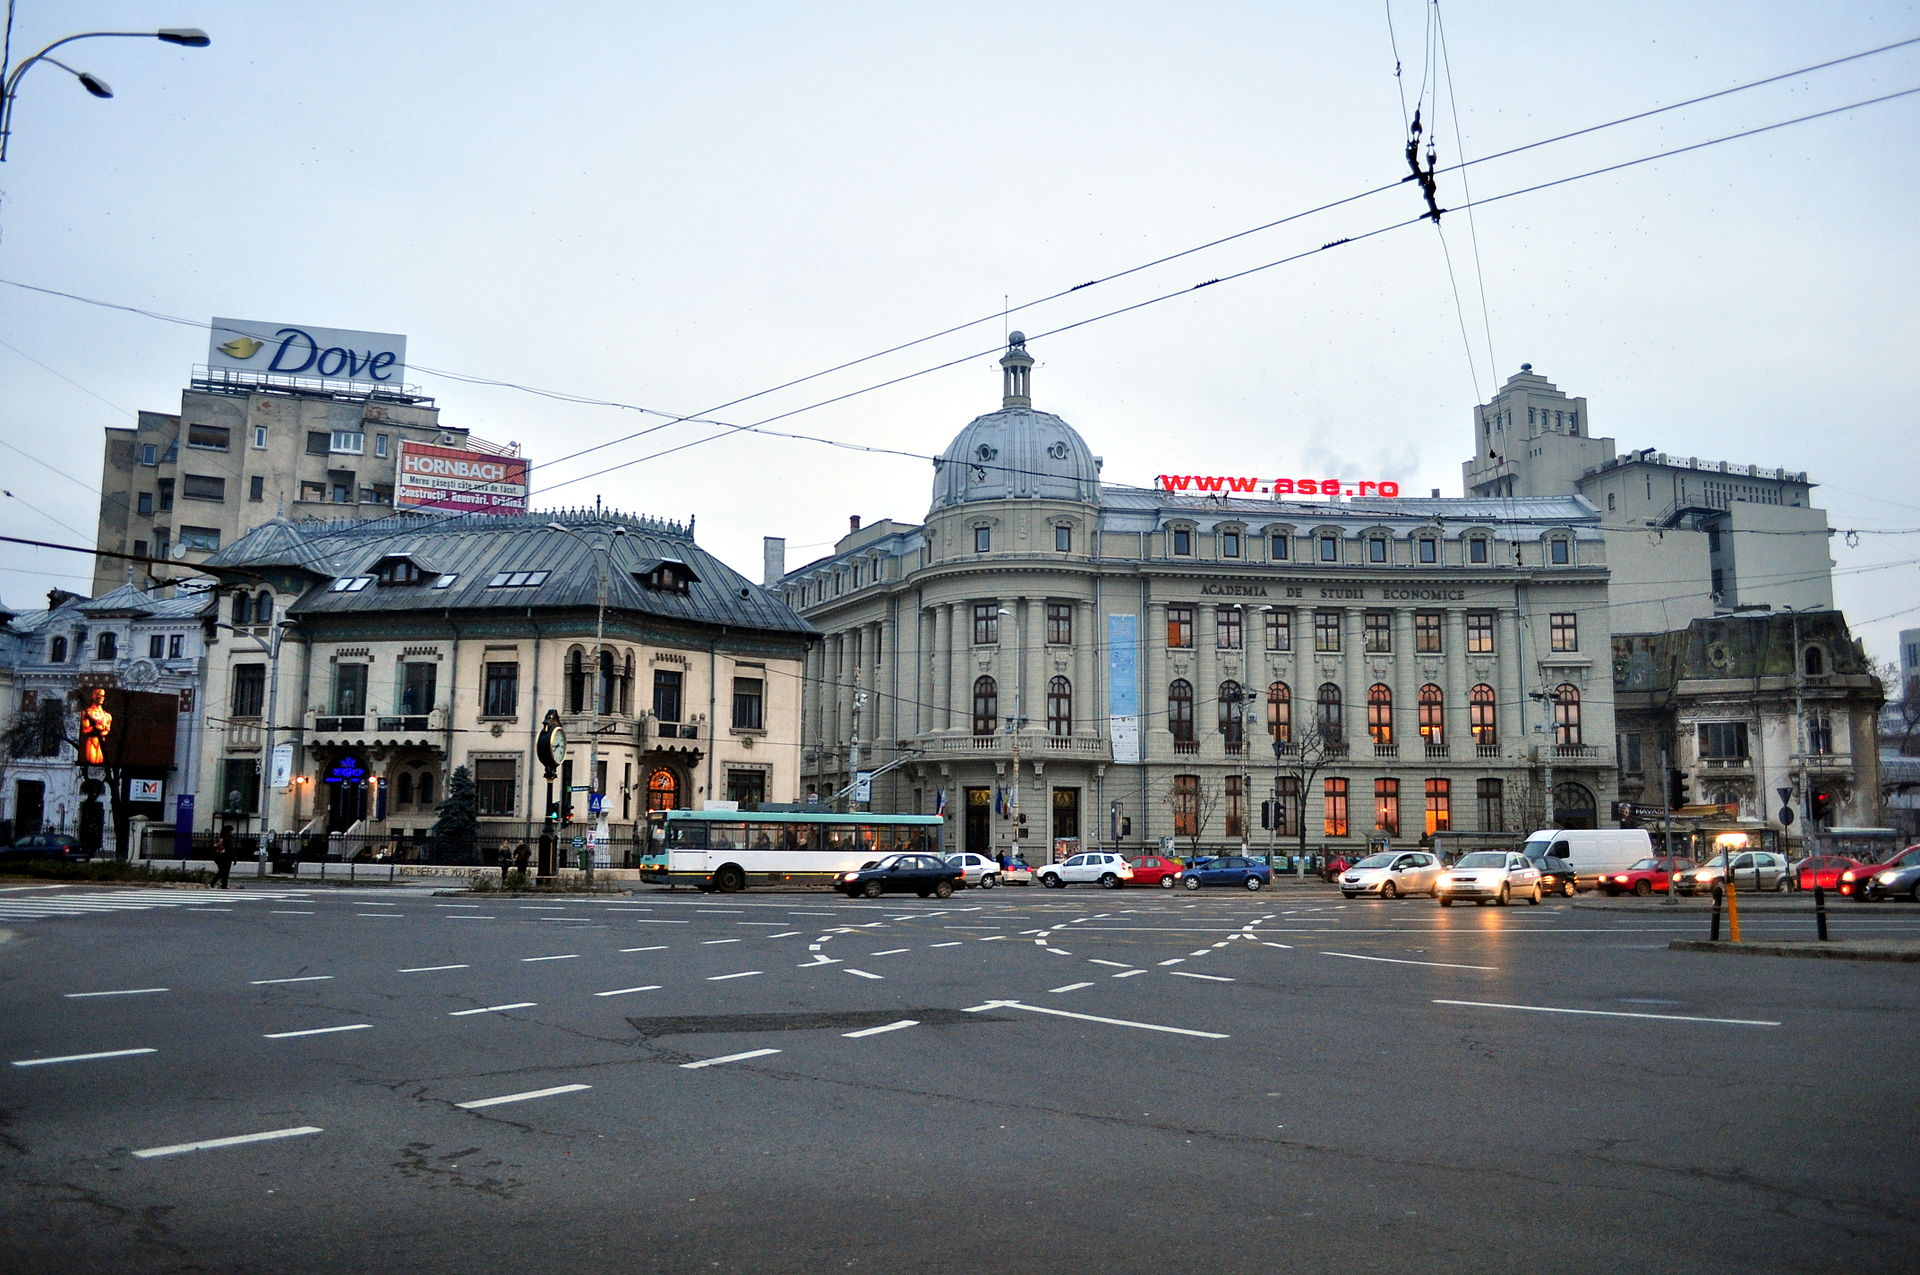
\includegraphics[height=0.40\textheight]{ch0_ase_2014.jpg}\\[1mm]
\imgcap{Bucharest University of Economic Studies}
\imgcredit{https://commons.wikimedia.org/wiki/File:Bucharest_-_Academie_de_Studii_Economice_01.jpg}{Photo: Joe Mabel (2014); CC BY 3.0; Wikimedia Commons}
\end{column}
\end{columns}
\end{frame}

\begin{frame}{Content Assessed}
\itemsize{\small}
\begin{itemize}
    \item \textbf{\sfmchlink{https://danpele.github.io/SFM/EN/Courses/chapter0_introduction.pdf}{Chapters 0}--\sfmchlink{https://danpele.github.io/SFM/EN/Courses/chapter15_systemic_risk.pdf}{15}}: lectures and seminars
    \begin{itemize}
        \item the definitions and formulas of the ``What You Need for Today'' slides of every seminar
        \item the computations of Part A of the seminars, on paper
    \end{itemize}
    \item \textbf{Reading software output}
    \begin{itemize}
        \item tables and charts like those of Part B: estimates, test statistics, $p$-values, backtests
        \item no code is written at the exam
    \end{itemize}
    \item \textbf{Understanding, not memory}
    \begin{itemize}
        \item why a method fails on financial returns, which test answers which question
    \end{itemize}
\end{itemize}
\end{frame}

\begin{frame}{Grading Criteria}
\itemsize{\small}
\begin{itemize}
    \item \textbf{The method}: the formula, with the numbers substituted
    \begin{itemize}
        \item a correct method with an arithmetic slip receives most of the points
    \end{itemize}
    \item \textbf{The result}: the number, with its unit (\%, days, RON) and its sign
    \begin{itemize}
        \item for a test: $H_0$, the statistic, the critical value or the $p$-value, the decision
    \end{itemize}
    \item \textbf{The interpretation}: three to five sentences, statistical and economic
    \begin{itemize}
        \item state the assumptions of an approximate formula (i.i.d., Normal, large $n$)
        \item a correct number with a wrong interpretation does not receive all the points
    \end{itemize}
\end{itemize}
\end{frame}

\begin{frame}{Typical Problem Types}
\itemsize{\small}
\begin{center}
\footnotesize
\begin{tabular}{>{\raggedright\arraybackslash}p{4.2cm}>{\raggedright\arraybackslash}p{1.4cm}>{\raggedright\arraybackslash}p{5.3cm}}
\toprule
\textbf{Type} & \textbf{Chapters} & \textbf{Example in this chapter} \\
\midrule
returns, annualisation, performance & 0, 1 & Problem 1: CAGR, drawdown, volatility drag \\
moments, normality, tails & 2, 3, 5, 6 & Problem 2: JB, Student-$t$, Hill \\
probability and simulation & 4 & Problem 3: portfolio, Monte Carlo, GBM \\
efficiency and memory & 7, 11 & Problems 4 and 7: Ljung--Box, VR, Hurst \\
volatility & 8, 9, 14 & Problem 5: GARCH, EWMA, annualisation of Bitcoin \\
risk measures and backtesting & 10 & Problem 6: VaR, ES, Kupiec, traffic light \\
credit and systemic risk & 12, 13, 15 & Problem 8: confusion matrix, EL, $\Delta$CoVaR \\
\bottomrule
\end{tabular}
\end{center}
\begin{itemize}
    \item The eight problems below are review examples with full solutions; the exam has its own subjects
\end{itemize}
\end{frame}

\begin{frame}{Problem 1: Returns and Drawdown}
\itemsize{\footnotesize}
\begin{itemize}
    \item \textbf{Context}
    \begin{itemize}
        \item An index is worth 100, 160, 64 and 96 at the end of years 0, 1, 2 and 3
    \end{itemize}
    \item \textbf{Tasks}
\begin{enumerate}
    \item Compute the simple returns $R_t$ and the log returns $r_t$ of the three years.
    \item Compute the total return in two ways: from $\sum_t r_t$ and from the prices.
    \item Compute the arithmetic mean of $R_t$ and the CAGR, and explain the difference.
    \item Compute the maximum drawdown and the gain needed from the trough to the previous peak.
\end{enumerate}
\end{itemize}
\end{frame}

\begin{frame}{Problem 1: Solution}
\itemsize{\footnotesize}
\begin{enumerate}
    \item $R = 60\%, -60\%, 50\%$; $r = \ln 1.6 = 0.470$, $\ln 0.4 = -0.916$, $\ln 1.5 = 0.405$
    \item $\sum_t r_t = -0.041 = \ln(96/100)$, so the total return is $e^{-0.041} - 1 = -4\%$, the same as $96/100 - 1$
    \item arithmetic mean $(60 - 60 + 50)/3 = 16.67\%$; CAGR $= (96/100)^{1/3} - 1 = -1.35\%$
    \item MDD $= 64/160 - 1 = -60\%$; to return from 64 to 160 the index needs $160/64 - 1 = 150\%$
\end{enumerate}
\begin{itemize}
    \item \textbf{Interpretation}
    \begin{itemize}
        \item A positive average return and a loss of money: volatility lowers the compound growth (volatility drag)
        \item Log returns add over time; simple returns do not
    \end{itemize}
\end{itemize}
\end{frame}

\begin{frame}{Problem 2: Distribution and Tails}
\itemsize{\footnotesize}
\begin{itemize}
    \item \textbf{Context}
    \begin{itemize}
        \item $n = 1000$ daily returns with skewness $S = -0.5$ and excess kurtosis $K = 6$
        \item The five largest losses, in \%: $8.2$, $6.5$, $5.9$, $5.1$, $4.6$; $\chi^2_{0.95}(2) = 5.99$
    \end{itemize}
    \item \textbf{Tasks}
\begin{enumerate}
    \item Compute the Jarque--Bera statistic, its two parts, and decide at 5\%.
    \item Find the degrees of freedom $\nu$ of a Student-$t$ distribution with the same excess kurtosis.
    \item Compute the Hill estimate $\hat\alpha$ with $k = 4$.
    \item Say which moments of the losses exist if $\alpha = \hat\alpha$, and whether a stable law with $\alpha < 2$ is consistent with it.
\end{enumerate}
\end{itemize}
\end{frame}

\begin{frame}{Problem 2: Solution}
\itemsize{\footnotesize}
\begin{enumerate}
    \item skewness part $\frac{1000}{6}(0.25) = 41.67$; kurtosis part $\frac{1000}{24}(36) = 1500.0$; JB $= 1541.7 > 5.99$: normality is rejected
    \item $6/(\nu - 4) = 6 \Rightarrow \nu = 5$
    \item $\ln(8.2/4.6) = 0.578$, $\ln(6.5/4.6) = 0.346$, $\ln(5.9/4.6) = 0.249$, $\ln(5.1/4.6) = 0.103$; mean $0.3190$, so $\hat\alpha = 3.14$
    \item moments of order $p < 3.14$ exist: mean, variance, skewness; the kurtosis does not; a stable law with $\alpha < 2$ (infinite variance) has heavier tails than these data
\end{enumerate}
\begin{itemize}
    \item \textbf{Interpretation}
    \begin{itemize}
        \item The kurtosis part dominates JB: heavy tails, not asymmetry, reject normality
        \item $k = 4$ gives a very noisy $\hat\alpha$ (SE $\approx \hat\alpha/2$); in practice $k$ is chosen from a Hill plot
    \end{itemize}
\end{itemize}
\end{frame}

\begin{frame}{Problem 3: Portfolio, Monte Carlo and GBM}
\itemsize{\footnotesize}
\begin{itemize}
    \item \textbf{Context}
    \begin{itemize}
        \item Two assets: daily volatilities $1.5\%$ and $2.5\%$, correlation $0.3$, weights 60\% and 40\%
        \item A share price follows a GBM with $\mu = 8\%$, $\sigma = 25\%$ a year, $S_0 = 100$
    \end{itemize}
    \item \textbf{Tasks}
\begin{enumerate}
    \item Compute the daily volatility of the portfolio and compare it with the weighted average of the volatilities.
    \item A Monte Carlo study with $N = 10\,000$ draws estimates a probability of 1\%; compute its SE and a 95\% interval.
    \item Compute the mean and the median of $S_1$, and $P(S_1 < S_0)$.
\end{enumerate}
\end{itemize}
\end{frame}

\begin{frame}{Problem 3: Solution}
\itemsize{\footnotesize}
\begin{enumerate}
    \item $\sigma_p^2 = 0.81 + 1.00 + 0.54 = 2.35$, $\sigma_p = 1.53\%$, below the weighted average $1.90\%$
    \item SE $= \sqrt{0.01 \times 0.99/10\,000} = 0.099\%$; interval $[0.80\%, 1.20\%]$
    \item mean $100e^{0.08} = 108.33$; median $100e^{0.08 - 0.03125} = 105.00$; $P(S_1 < S_0) = \Phi(-0.0488/0.25) = \Phi(-0.195) = 42.3\%$
\end{enumerate}
\begin{itemize}
    \item \textbf{Interpretation}
    \begin{itemize}
        \item Diversification: with $\rho < 1$ the portfolio is less risky than the average of its parts
        \item A GBM investor loses money after one year with probability 42.3\%, although the expected price rises
    \end{itemize}
\end{itemize}
\end{frame}

\begin{frame}{Problem 4: Autocorrelation and the Variance Ratio}
\itemsize{\footnotesize}
\begin{itemize}
    \item \textbf{Context}
    \begin{itemize}
        \item $T = 2500$ daily returns; $\hat\rho(1) = 0.06$, $\hat\rho(2) = 0.02$, $\hat\rho(3) = -0.01$, $\hat\rho(4) = 0.01$; $\chi^2_{0.95}(4) = 9.49$
        \item The heteroskedasticity-robust standard error of $\widehat{\mathrm{VR}}(5)$ is $0.065$
    \end{itemize}
    \item \textbf{Tasks}
\begin{enumerate}
    \item Compute the Ljung--Box statistic $Q(4)$ and decide at 5\%.
    \item Compute $\mathrm{VR}(5) = 1 + 2\sum_{k=1}^{4}(1 - k/5)\hat\rho(k)$.
    \item Compute the i.i.d. statistic $Z(5)$ with SE $= \sqrt{2(2q-1)(q-1)/(3qT)}$ and the robust $Z^*(5)$, and decide at 5\%.
\end{enumerate}
\end{itemize}
\end{frame}

\begin{frame}{Problem 4: Solution}
\itemsize{\footnotesize}
\begin{enumerate}
    \item $Q(4) = T(T+2)\sum_{k=1}^{4}\hat\rho_k^2/(T-k) = 10.51$, close to $T\sum_k\hat\rho_k^2$ with $\sum_k\hat\rho_k^2 = 0.0042$; $10.51 > 9.49$: the absence of autocorrelation is rejected
    \item $\mathrm{VR}(5) = 1 + 2(0.8 \times 0.06 + 0.6 \times 0.02 - 0.4 \times 0.01 + 0.2 \times 0.01) = 1 + 2 \times 0.058 = 1.116$
    \item SE $= \sqrt{72/37\,500} = 0.0438$, $Z(5) = 2.65 > 1.96$; robust $Z^*(5) = (1.116 - 1)/0.065 = 1.78 < 1.96$
\end{enumerate}
\begin{itemize}
    \item \textbf{Interpretation}
    \begin{itemize}
        \item VR $> 1$: positive autocorrelation (momentum); the i.i.d. test rejects the random walk
        \item The robust test does not: volatility clustering inflates $Z(5)$; the robust decision is the one to report
    \end{itemize}
\end{itemize}
\end{frame}

\begin{frame}{Problem 5: Volatility Forecasts}
\itemsize{\footnotesize}
\begin{itemize}
    \item \textbf{Context}
    \begin{itemize}
        \item GARCH(1,1) for daily returns in \%: $\omega = 0.03$, $\alpha = 0.09$, $\beta = 0.89$; today $\sigma_t^2 = 1.8$ and $\varepsilon_t = -2.5$
        \item Bitcoin: daily standard deviation $3.5\%$
    \end{itemize}
    \item \textbf{Tasks}
\begin{enumerate}
    \item Compute $\sigma_{t+1}^2$ and the one-day Normal VaR 1\% (mean zero, $z_{0.01} = -2.326$).
    \item Compute the persistence, the half-life, the long-run variance and the long-run annual volatility.
    \item Compute $E_t[\sigma_{t+10}^2]$ and the EWMA forecast with $\lambda = 0.94$.
    \item Annualise the volatility of Bitcoin.
\end{enumerate}
\end{itemize}
\end{frame}

\begin{frame}{Problem 5: Solution}
\itemsize{\footnotesize}
\begin{enumerate}
    \item $\sigma_{t+1}^2 = 0.03 + 0.5625 + 1.602 = 2.1945$, $\sigma_{t+1} = 1.481\%$; VaR 1\% $= 2.326 \times 1.481 = 3.45\%$
    \item $\alpha + \beta = 0.98$; $h_{1/2} = \ln 0.5/\ln 0.98 = 34.3$ days; $\bar\sigma^2 = 0.03/0.02 = 1.50$; $\sqrt{252 \times 1.50} = 19.44\%$ a year
    \item $E_t\sigma_{t+10}^2 = 1.50 + 0.98^9(2.1945 - 1.50) = 2.079$; EWMA: $0.94 \times 1.8 + 0.06 \times 6.25 = 2.067$
    \item Bitcoin trades every day: $3.5 \times \sqrt{365} = 66.9\%$; with 252 the result, $55.6\%$, would be wrong
\end{enumerate}
\begin{itemize}
    \item \textbf{Interpretation}
    \begin{itemize}
        \item A large negative shock raises tomorrow's variance; the forecast returns to $\bar\sigma^2$ at the speed $\alpha + \beta$
        \item EWMA has no long-run level: its forecast stays flat for every horizon
    \end{itemize}
\end{itemize}
\end{frame}

\begin{frame}{Problem 6: VaR, ES and Backtesting}
\itemsize{\footnotesize}
\begin{itemize}
    \item \textbf{Context}
    \begin{itemize}
        \item A position of 1\,000\,000 RON; daily returns $N(0, 1.6^2)$ in \%; $\varphi(1.96) = 0.0584$
        \item The seven smallest of 250 historical returns, in \%: $-5.1$, $-4.4$, $-3.9$, $-3.6$, $-3.2$, $-3.0$, $-2.9$
    \end{itemize}
    \item \textbf{Tasks}
\begin{enumerate}
    \item Compute the Normal VaR 1\% and ES 2.5\% in \% and in RON, and the 10-day VaR 1\% by the square-root-of-time rule.
    \item Compute VaR 1\% and ES 2.5\% by historical simulation.
    \item A model has 6 exceptions of VaR 1\% in 250 days: compute the Kupiec statistic, decide at 5\%, and give the Basel zone.
\end{enumerate}
\end{itemize}
\end{frame}

\begin{frame}{Problem 6: Solution}
\itemsize{\footnotesize}
\begin{enumerate}
    \item VaR 1\% $= 2.326 \times 1.6 = 3.72\%$ (37\,222 RON); ES 2.5\% $= 1.6 \times 0.0584/0.025 = 1.6 \times 2.338 = 3.74\%$ (37\,405 RON); 10 days: $\sqrt{10} \times 3.72 = 11.77\%$
    \item $k = \lceil 2.5 \rceil = 3$: VaR 1\% $= 3.9\%$; $k = \lceil 6.25 \rceil = 7$: ES 2.5\% $= 26.1/7 = 3.73\%$
    \item $\ell_0 = 244\ln 0.99 + 6\ln 0.01 = -30.08$, $\ell_1 = 244\ln 0.976 + 6\ln 0.024 = -28.31$; $LR_{uc} = 3.56 < 3.84$ ($p = 0.059$): not rejected; yellow zone (5--9 exceptions)
\end{enumerate}
\begin{itemize}
    \item \textbf{Interpretation}
    \begin{itemize}
        \item For the Normal distribution ES 2.5\% and VaR 1\% are almost equal; the historical tail is heavier
        \item Kupiec does not reject 6 exceptions, but the traffic light already asks for a higher capital multiplier
    \end{itemize}
\end{itemize}
\end{frame}

\begin{frame}{Problem 7: Long Memory and Risk Scaling}
\itemsize{\footnotesize}
\begin{itemize}
    \item \textbf{Context}
    \begin{itemize}
        \item The average R/S statistic of daily returns is $4.1$ for blocks of $n = 20$ days and $60.0$ for $n = 2000$
        \item One-day VaR 1\% $= 2.5\%$
    \end{itemize}
    \item \textbf{Tasks}
\begin{enumerate}
    \item Estimate $H$ from the slope of $\log(R/S)$ on $\log n$, and the fractional parameter $d$.
    \item Scale the VaR to 10 days with $h^H$ and with $\sqrt{h}$, and compare.
    \item Say what must be checked before concluding that there is long memory.
\end{enumerate}
\end{itemize}
\end{frame}

\begin{frame}{Problem 7: Solution}
\itemsize{\footnotesize}
\begin{enumerate}
    \item $H = \log_{10}(60.0/4.1)/\log_{10}(2000/20) = \log_{10}(14.63)/2 = 1.165/2 = 0.583$; $d = H - 0.5 = 0.083$
    \item $10^{H} = 3.83$: VaR $= 9.56\%$; $\sqrt{10} = 3.16$: VaR $= 7.91\%$
    \item a Monte Carlo band of $\hat H$ for i.i.d. data of the same length (R/S is biased upwards), the Lo test, split samples and shuffled data (breaks, GARCH)
\end{enumerate}
\begin{itemize}
    \item \textbf{Interpretation}
    \begin{itemize}
        \item With $H > 0.5$ the square-root-of-time rule understates multi-day risk
        \item On the course data the long memory is in $|r_t|$, not in $r_t$ (\sfmchlink{https://danpele.github.io/SFM/EN/Courses/chapter11_fractal_markets_long_memory.pdf}{Chapter 11})
    \end{itemize}
\end{itemize}
\end{frame}

\begin{frame}{Problem 8: Credit Scoring and Systemic Risk}
\itemsize{\footnotesize}
\begin{itemize}
    \item \textbf{Context}
    \begin{itemize}
        \item A test sample of 300 loans, 90 bad; at the chosen cut-off: 60 bad and 42 good loans are flagged as bad
        \item Quantile regression at 1\% of the system return on a bank's return: $\hat a = -2.1$, $\hat b = 0.6$; bank: $q_{0.01} = -5.0\%$, median $0.1\%$
    \end{itemize}
    \item \textbf{Tasks}
\begin{enumerate}
    \item Compute the accuracy, the true positive rate (TPR), the false positive rate (FPR) and the precision, and compare the accuracy with ``always good''.
    \item Compute the Gini coefficient for AUC $= 0.80$ and the expected loss for PD $= 4\%$, LGD $= 45\%$, EAD $= 200\,000$ RON.
    \item Compute the CoVaR 1\% of the system with the bank at its VaR and at its median, and $\Delta$CoVaR.
\end{enumerate}
\end{itemize}
\end{frame}

\begin{frame}{Problem 8: Solution}
\itemsize{\footnotesize}
\begin{enumerate}
    \item accuracy $(60 + 168)/300 = 76.0\%$; TPR $= 60/90 = 66.7\%$; FPR $= 42/210 = 20.0\%$; precision $60/102 = 58.8\%$; ``always good'': 70.0\%
    \item Gini $= 2 \times 0.80 - 1 = 0.60$; EL $= 0.04 \times 0.45 \times 200\,000 = 3\,600$ RON
    \item CoVaR $= -(-2.1 + 0.6 \times (-5.0)) = 5.10\%$; at the median: $-(-2.1 + 0.6 \times 0.1) = 2.04\%$; $\Delta$CoVaR $= 0.6 \times 5.1 = 3.06$ pp
\end{enumerate}
\begin{itemize}
    \item \textbf{Interpretation}
    \begin{itemize}
        \item The model is barely more accurate than ``always good'', but it finds two thirds of the bad loans: judge it by AUC and costs
        \item The distress of this bank raises the VaR of the system by 3.06 percentage points
    \end{itemize}
\end{itemize}
\end{frame}

\begin{frame}{Recap: The Exam}
\itemsize{\small}
\begin{itemize}
    \item Written, 2 hours, calculator allowed; \sfmchlink{https://danpele.github.io/SFM/EN/Courses/chapter0_introduction.pdf}{Chapters 0}--\sfmchlink{https://danpele.github.io/SFM/EN/Courses/chapter15_systemic_risk.pdf}{15}; computations and interpretations
    \item Points for the method, the result with its unit and sign, and the interpretation
    \item Practise with Part A of every seminar and with the review seminar
\end{itemize}
\end{frame}


%=============================================================================
\section{The Team Project}
%=============================================================================

\begin{frame}{The Team Project: Content and Deliverables}
\itemsize{\small}
\begin{itemize}
    \item \textbf{20\% of the final grade}: a team analysis of real market data with the methods of the course
    \begin{itemize}
        \item one research question; returns and indicators, distributions and tails, efficiency tests, volatility and risk measures
        \item ideas: the ``Project Idea'' slide at the end of every chapter and Part C of every seminar
    \end{itemize}
    \item \textbf{Deliverables}
    \begin{itemize}
        \item a GitHub repository whose code reproduces every number and every chart from the saved data
        \item a short report and a presentation of the results
        \item the file \texttt{AI\_USE.md}, which declares every use of AI tools
    \end{itemize}
\end{itemize}
\end{frame}

\begin{frame}{Project Grading Criteria}
\itemsize{\small}
\begin{itemize}
    \item \textbf{The question}: clear, answerable with the data, relevant for investors or regulators
    \begin{itemize}
        \item ``Is the BET today less volatile than in 2008?'' is a question; ``an analysis of the BET'' is not
    \end{itemize}
    \item \textbf{The methods and the checks}
    \begin{itemize}
        \item the right test for the question (the toolbox); robust standard errors; out-of-sample evaluation
        \item robustness: another window, another series, another estimator
    \end{itemize}
    \item \textbf{The interpretation}: what the numbers mean, and what the data cannot show
    \begin{itemize}
        \item \textbf{Reproducibility}: the repository runs from the saved data to every chart
    \end{itemize}
\end{itemize}
\end{frame}

\begin{frame}{The Oral Defence}
\itemsize{\small}
\begin{itemize}
    \item \textbf{Each member explains the code and the results}
    \begin{itemize}
        \item typical questions: what does this line compute? where does this number come from? why this test and not another?
        \item what changes if the window, the series or the level $\alpha$ changes?
    \end{itemize}
    \item \textbf{A line of code that cannot be explained does not count as your own work}
    \begin{itemize}
        \item this holds for code written with or without AI
    \end{itemize}
    \item \textbf{Preparation}
    \begin{itemize}
        \item rerun the repository from scratch the day before; know the definitions of every number on your slides
    \end{itemize}
\end{itemize}
\end{frame}

\begin{frame}{The File AI\_USE.md}
\itemsize{\small}
\begin{itemize}
    \item \textbf{AI tools are allowed and must be declared}
    \begin{itemize}
        \item for every use: the tool, the prompt, what was kept and what was corrected
        \item the errors of the AI that you found and how you found them
    \end{itemize}
    \item \textbf{You are responsible for every number and every reference}
    \begin{itemize}
        \item every number: recomputed with your own code from the course data
        \item every reference: its DOI opened and its title checked
    \end{itemize}
    \item \textbf{Typical AI errors in this course}
    \begin{itemize}
        \item ``VaR 99\%'' with a negative sign, Bitcoin annualised with 252 days, invented references, a test with the wrong distribution
    \end{itemize}
\end{itemize}
\end{frame}

\begin{frame}{Recap: The Team Project}
\itemsize{\small}
\begin{itemize}
    \item One question, real data, reproducible code, a short report, a presentation
    \item Graded on the question, the methods and checks, the interpretation and the oral defence
    \item AI allowed, declared in \texttt{AI\_USE.md}, every number and reference checked
\end{itemize}
\end{frame}


%=============================================================================
\section{How AI Could Help: Your Own Research}
%=============================================================================

\begin{frame}{An Open Question for Your Own Research}
\itemsize{\small}
\begin{columns}[T]
\begin{column}{0.60\textwidth}
\begin{itemize}
    \item \textbf{Has the BET become a ``normal'' market?}
    \begin{itemize}
        \item since 1997: VR(5) $= 1.28$ (momentum) and tail index 2.57
        \item since 2015: VR(5) $= 1.17$, $Z^* = 1.93$, tail index 2.19
    \end{itemize}
    \item \textbf{Why it is open}
    \begin{itemize}
        \item the momentum fades, but the tails do not become thinner
        \item one extreme day ($-11.9\%$ on 19 December 2018) moves the tail estimate; few crises, short samples
    \end{itemize}
    \item Different teams with the same data reach different answers: nonstandard errors \refMenk
\end{itemize}
\end{column}
\begin{column}{0.36\textwidth}
\centering
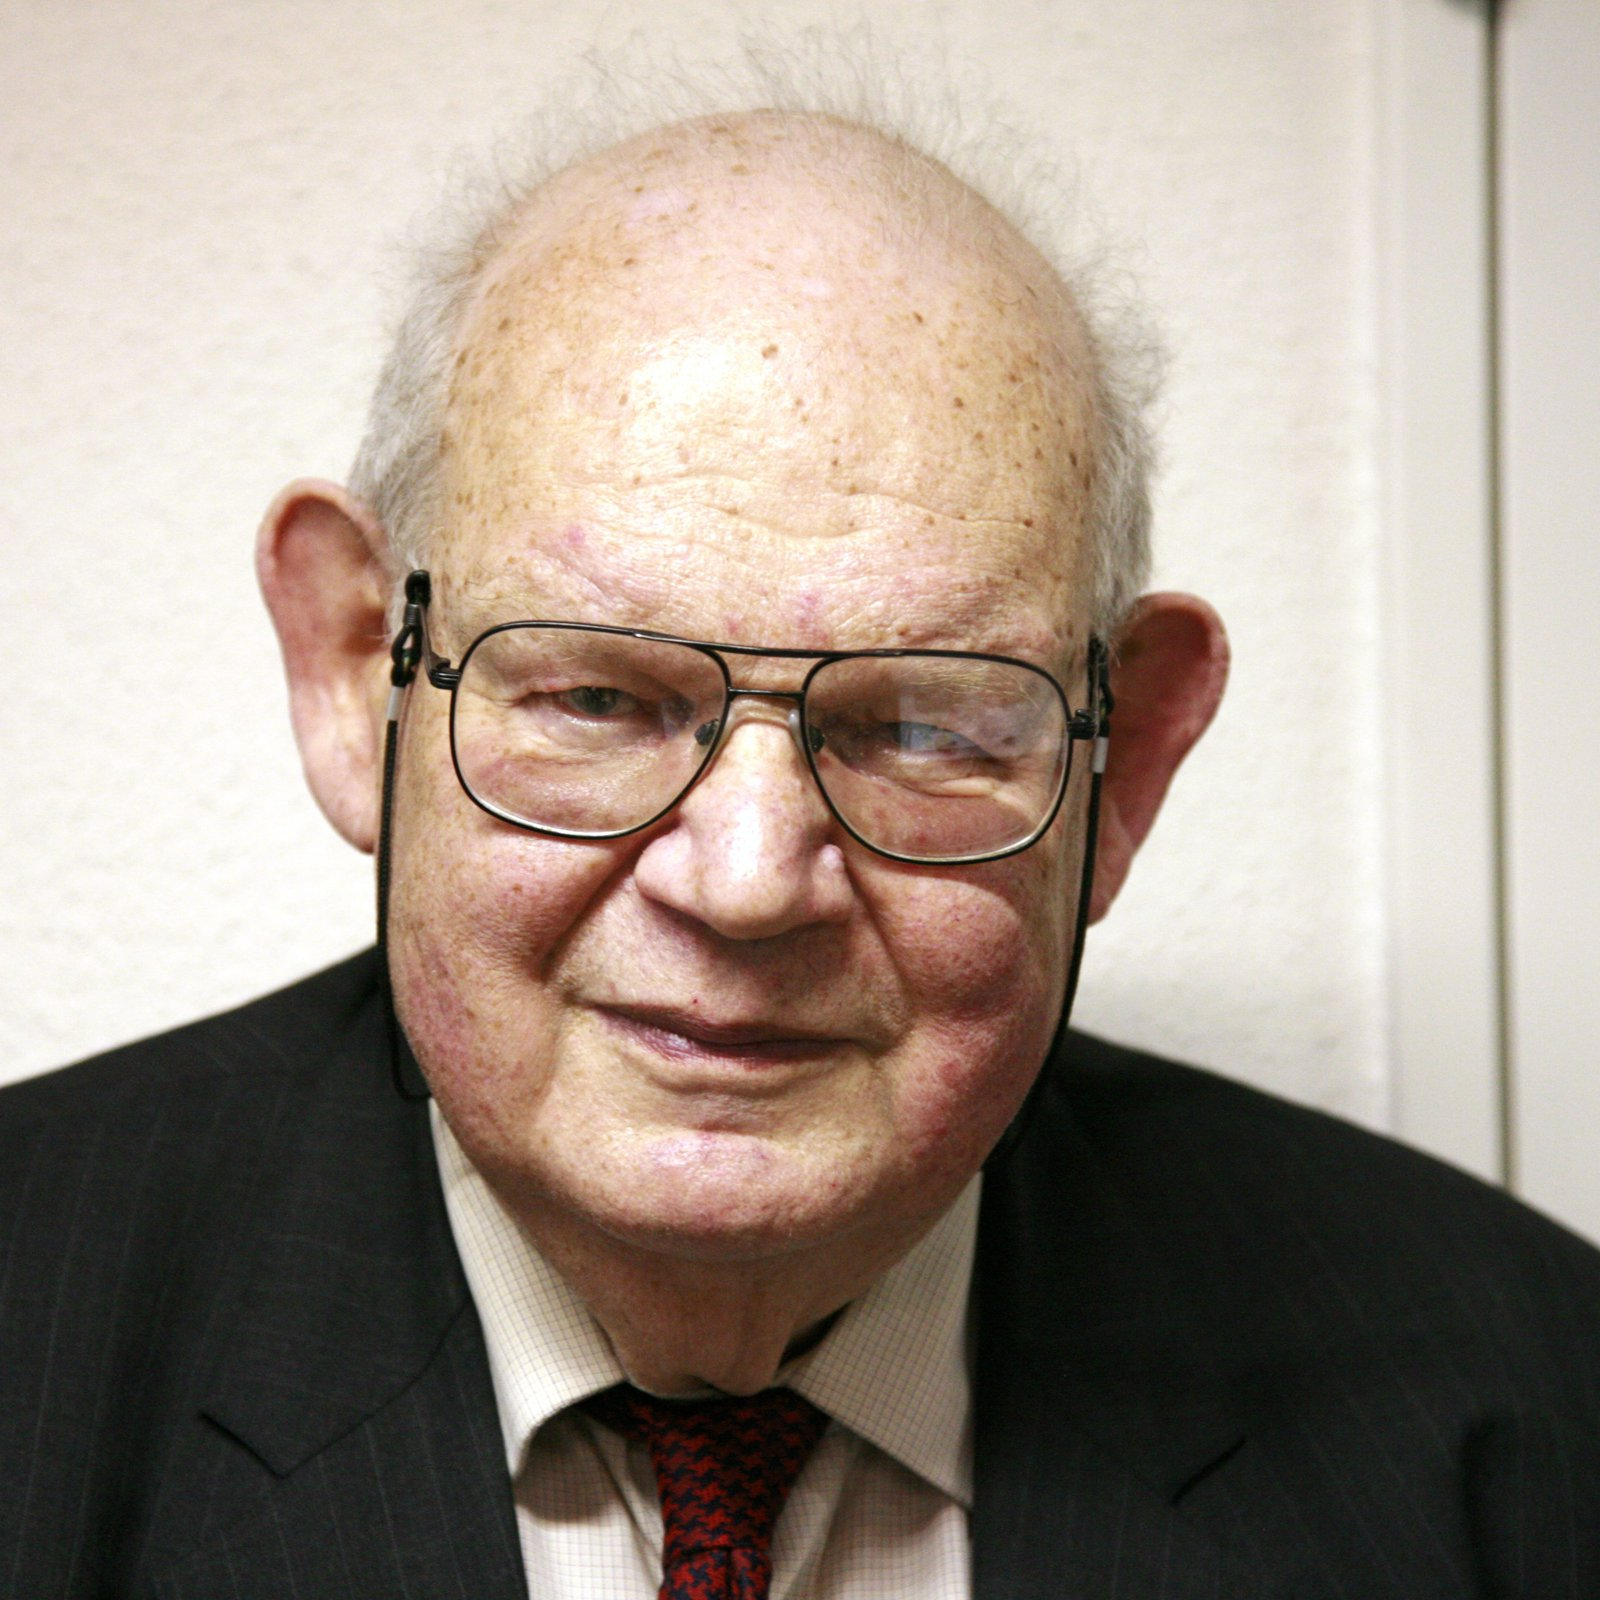
\includegraphics[height=0.40\textheight]{ch0_mandelbrot_2007.jpg}\\[1mm]
\imgcap{Benoit Mandelbrot, who showed in 1963 that price changes have heavy tails}
\imgcredit{https://commons.wikimedia.org/wiki/File:Benoit_Mandelbrot_mg_1804-d.jpg}{Photo: Rama (2007); CC BY-SA 2.0 fr; Wikimedia Commons}
\end{column}
\end{columns}
\end{frame}

\begin{frame}{The Research Loop}
\itemsize{\small}
\begin{enumerate}
    \item \textbf{Question}: one sentence, with a number that would answer it
    \item \textbf{Data}: series, source, calendar, window, fixed before looking at the results
    \item \textbf{Method}: the test from the toolbox, with its null hypothesis
    \item \textbf{Checks}: robust SE, Monte Carlo band, subsamples, another estimator
    \item \textbf{Interpretation}: the answer, its uncertainty, its limits
    \item \textbf{Replication}: a second person runs the code and gets the same numbers
\end{enumerate}
\begin{itemize}
    \item AI can speed up every step; it replaces none of the checks \refWang
\end{itemize}
\end{frame}

\begin{frame}{How AI Could Help}
\itemsize{\small}
\begin{itemize}
    \item \textbf{Literature}: a first list of studies on the efficiency and the tails of emerging markets, each to be checked by its DOI
    \item \textbf{Code}: a first draft of rolling VR(5), Hill and GARCH estimates on windows of 500 days
    \item \textbf{Robustness}: a grid of choices (window, $k$, level $\alpha$, series) and one table of all results
    \item \textbf{Writing}: a clearer paragraph, after the numbers are final
    \item Example prompt
    \begin{itemize}
        \item \aiprompt{Write Python code that computes, on rolling windows of 500 trading days moved by 21 days, the Lo-MacKinlay robust variance-ratio statistic Z*(5), the Hill tail index of the losses with k = 2.5\% of the window, and the GARCH(1,1)-t persistence for the daily log returns of the BET, and plots the three series with their 95\% bands.}
    \end{itemize}
\end{itemize}
\end{frame}

\begin{frame}{What to Check}
\itemsize{\small}
\begin{itemize}
    \item The formulas: the robust $Z^*(q)$, not $Z(q)$; the Hill estimator on losses $L = -r$, with $k$ given as a share of the window
    \item The look-ahead: each window uses only the data up to its last day
    \item The bands: overlapping windows are not independent evidence; one result in twenty is significant by chance
    \item The numbers: recompute one window step by step and compare
    \item The references: every cited paper must exist; open the DOI and check the title
\end{itemize}
\end{frame}

\begin{frame}{Project Idea}
\itemsize{\small}
\begin{itemize}
    \item \textbf{Question}: did the BET become more efficient, less volatile and thinner-tailed between 2000 and 2026?
    \begin{itemize}
        \item data: BET since 1997, with the S\&P 500 and the DAX as benchmarks (EODHD)
    \end{itemize}
    \item Steps
    \begin{itemize}
        \item rolling robust VR(5), Hill index, GARCH persistence and Hurst exponent (\sfmchlink{https://danpele.github.io/SFM/EN/Courses/chapter5_heavy_tails_evt.pdf}{Chapters 5}, \sfmchlink{https://danpele.github.io/SFM/EN/Courses/chapter7_efficient_markets_random_walk_vr.pdf}{7}, \sfmchlink{https://danpele.github.io/SFM/EN/Courses/chapter9_arch_garch_models.pdf}{9}, \sfmchlink{https://danpele.github.io/SFM/EN/Courses/chapter11_fractal_markets_long_memory.pdf}{11})
        \item bands from Monte Carlo or the bootstrap; the same analysis for the benchmarks
        \item dates of change (e.g.\ 2008, 2020) checked against the bands, not chosen after looking
    \end{itemize}
    \item Deliverable: one chart with four panels, one table, and a paragraph on what the data can and cannot show
    \item Declare any AI use, and list the errors of the AI that you corrected
\end{itemize}
\end{frame}


%=============================================================================
\section{Summary}
%=============================================================================

\begin{frame}{Key Takeaways}
\itemsize{\small}
\begin{itemize}
    \item Returns, not prices: log returns in \%, the right calendar, annualised with the actual frequency
    \item Returns have heavy tails (tail index 2--4), negative skewness and finite variance: the Normal distribution understates risk
    \item The sign of returns is almost unpredictable; their size is predictable (volatility clustering, GARCH)
    \item Risk: VaR 1\% $= -q_{1\%}$ and ES 2.5\%, always followed by a backtest
    \item Every result needs its uncertainty: SE, robust tests, Monte Carlo bands, out-of-sample checks
    \item The exam rewards method, result and interpretation; the project rewards a clear question answered honestly
\end{itemize}
\end{frame}

\begin{frame}{Check Yourself}
\itemsize{\small}
\begin{itemize}
    \item \textbf{Question}: Ljung--Box does not reject on $r_t$ but rejects strongly on $r_t^2$. What does this mean?
    \begin{itemize}
        \item \textbf{Answer}: returns are uncorrelated but not independent: volatility clustering; model the variance (GARCH)
    \end{itemize}
    \item \textbf{Question}: a fitted stable law gives $\hat\alpha = 1.5$ and the Hill estimate is $\hat\alpha = 3$. Which is right about the variance?
    \begin{itemize}
        \item \textbf{Answer}: Hill, which looks only at the tail: the variance is finite; the stable fit describes the body
    \end{itemize}
    \item \textbf{Question}: a model has 1\% exceptions, all in March 2020. Is it a good VaR model?
    \begin{itemize}
        \item \textbf{Answer}: no: the rate is right, but the exceptions cluster; the Christoffersen test rejects it
    \end{itemize}
\end{itemize}
\end{frame}


%=============================================================================
\section{References}
%=============================================================================

\begin{frame}{References (1/2)}
\itemsize{\tiny}
\begin{itemize}
    \item Adrian, T., Brunnermeier, M.K. (2016). \href{https://doi.org/10.1257/aer.20120555}{CoVaR}. \textit{American Economic Review}, 106(7), 1705--1741.
    \item Altman, E.I. (1968). \href{https://doi.org/10.1111/j.1540-6261.1968.tb00843.x}{Financial ratios, discriminant analysis and the prediction of corporate bankruptcy}. \textit{Journal of Finance}, 23(4), 589--609.
    \item Artzner, P., Delbaen, F., Eber, J.-M., Heath, D. (1999). \href{https://doi.org/10.1111/1467-9965.00068}{Coherent measures of risk}. \textit{Mathematical Finance}, 9(3), 203--228.
    \item Bollerslev, T. (1986). \href{https://doi.org/10.1016/0304-4076(86)90063-1}{Generalized autoregressive conditional heteroskedasticity}. \textit{Journal of Econometrics}, 31(3), 307--327.
    \item Borak, S., Härdle, W.K., López-Cabrera, B. (2013). \href{https://doi.org/10.1007/978-3-642-33929-5}{\textit{Statistics of Financial Markets: Exercises and Solutions}}, 2nd ed. Springer.
    \item Campbell, J.Y., Lo, A.W., MacKinlay, A.C. (1997). \href{https://doi.org/10.1515/9781400830213}{\textit{The Econometrics of Financial Markets}}. Princeton University Press.
    \item Cont, R. (2001). \href{https://doi.org/10.1080/713665670}{Empirical properties of asset returns: stylized facts and statistical issues}. \textit{Quantitative Finance}, 1(2), 223--236.
    \item Diebold, F.X., Yilmaz, K. (2012). \href{https://doi.org/10.1016/j.ijforecast.2011.02.006}{Better to give than to receive: predictive directional measurement of volatility spillovers}. \textit{International Journal of Forecasting}, 28(1), 57--66.
    \item Engle, R.F. (1982). \href{https://doi.org/10.2307/1912773}{Autoregressive conditional heteroscedasticity with estimates of the variance of United Kingdom inflation}. \textit{Econometrica}, 50(4), 987--1007.
    \item Fama, E.F. (1970). \href{https://doi.org/10.2307/2325486}{Efficient capital markets: a review of theory and empirical work}. \textit{Journal of Finance}, 25(2), 383--417.
    \item Franke, J., Härdle, W.K., Hafner, C.M. (2019). \href{https://doi.org/10.1007/978-3-030-13751-9}{\textit{Statistics of Financial Markets: An Introduction}}, 5th ed. Springer.
    \item Gu, S., Kelly, B., Xiu, D. (2020). \href{https://doi.org/10.1093/rfs/hhaa009}{Empirical asset pricing via machine learning}. \textit{Review of Financial Studies}, 33(5), 2223--2273.
    \item Hill, B.M. (1975). \href{https://doi.org/10.1214/aos/1176343247}{A simple general approach to inference about the tail of a distribution}. \textit{Annals of Statistics}, 3(5), 1163--1174.
    \item Hurst, H.E. (1951). \href{https://doi.org/10.1061/TACEAT.0006518}{Long-term storage capacity of reservoirs}. \textit{Transactions of the American Society of Civil Engineers}, 116(1), 770--799.
    \item J.P. Morgan/Reuters (1996). \href{https://www.msci.com/documents/10199/5915b101-4206-4ba0-aee2-3449d5c7e95a}{\textit{RiskMetrics -- Technical Document}}, 4th ed. New York.
    \item Jarque, C.M., Bera, A.K. (1980). \href{https://doi.org/10.1016/0165-1765(80)90024-5}{Efficient tests for normality, homoscedasticity and serial independence of regression residuals}. \textit{Economics Letters}, 6(3), 255--259.
\end{itemize}
\end{frame}

\begin{frame}{References (2/2)}
\itemsize{\tiny}
\begin{itemize}
    \item Kupiec, P.H. (1995). \href{https://doi.org/10.3905/jod.1995.407942}{Techniques for verifying the accuracy of risk measurement models}. \textit{Journal of Derivatives}, 3(2), 73--84.
    \item Lo, A.W., MacKinlay, A.C. (1988). \href{https://doi.org/10.1093/rfs/1.1.41}{Stock market prices do not follow random walks: evidence from a simple specification test}. \textit{Review of Financial Studies}, 1(1), 41--66.
    \item Mandelbrot, B. (1963). \href{https://doi.org/10.1086/294632}{The variation of certain speculative prices}. \textit{Journal of Business}, 36(4), 394--419.
    \item McNeil, A.J., Frey, R., Embrechts, P. (2015). \href{https://press.princeton.edu/books/hardcover/9780691166278/quantitative-risk-management}{\textit{Quantitative Risk Management: Concepts, Techniques and Tools}}, revised ed. Princeton University Press.
    \item Menkveld, A.J., Dreber, A., Holzmeister, F., Huber, J., Johannesson, M., et al. (2024). \href{https://doi.org/10.1111/jofi.13337}{Nonstandard errors}. \textit{Journal of Finance}, 79(3), 2339--2390.
    \item Nakamoto, S. (2008). \href{https://bitcoin.org/bitcoin.pdf}{Bitcoin: a peer-to-peer electronic cash system}. White paper.
    \item Nolan, J.P. (2020). \href{https://doi.org/10.1007/978-3-030-52915-4}{\textit{Univariate Stable Distributions: Models for Heavy Tailed Data}}. Springer.
    \item Peters, E.E. (1994). \href{https://www.wiley.com/en-us/Fractal+Market+Analysis\%3A+Applying+Chaos+Theory+to+Investment+and+Economics-p-9780471585244}{\textit{Fractal Market Analysis: Applying Chaos Theory to Investment and Economics}}. Wiley.
    \item Tsay, R.S. (2010). \href{https://doi.org/10.1002/9780470644560}{\textit{Analysis of Financial Time Series}}, 3rd ed. Wiley.
    \item Wang, H., Fu, T., Du, Y., Gao, W., et al. (2023). \href{https://doi.org/10.1038/s41586-023-06221-2}{Scientific discovery in the age of artificial intelligence}. \textit{Nature}, 620, 47--60.
\end{itemize}
\end{frame}

\end{document}
